% !TeX root = ../notes.tex
% Planning version: section skeleton, content bullets, live TikZ, figure list, and reading list.
% This file is deliberately not final student prose.

\chapter{Modelling chemical reactivity}

\begin{notebox}
  \keypoint{What do you need to learn from this chapter?}
  Molecular descriptors become useful for prediction only when they are connected to a defined chemical response, a defensible dataset, and an appropriate model.
  This chapter develops the physical-organic idea of relating structure to reactivity or selectivity, then asks how far a fitted relationship can be interpreted and trusted.
\end{notebox}

\section{From describing molecules to modelling chemistry}

Chapter~4 represented molecules as points in chemical space.
That description did not require a measured chemical outcome because the objective was to compare molecules, visualise their relationships, and choose representative examples.
A reactivity model introduces a response such as rate, conversion, yield, regioselectivity, or enantioselectivity.
For $n$ experiments described by $p$ features, the inputs can be collected in an $(n, p)$ descriptor matrix $\mathbf{X}$ and the measured responses in a vector $\mathbf{y}$.
A fitted model tries to predict  $\hat{\mathbf{y}}=f(\mathbf{X})$.

\solution{7.0cm}{%
  \centering
  \resizebox{0.94\linewidth}{!}{%
    \begin{tikzpicture}[
      box/.style={draw=darkBlue,fill=paleBlue,line width=1.6pt,minimum width=3.5cm,minimum height=1.1cm,align=center,font=\sffamily},
      response/.style={draw=darkGreen,fill=paleGreen,line width=1.6pt,minimum width=3.5cm,minimum height=1.1cm,align=center,font=\sffamily},
      arrow/.style={->,>=Stealth,draw=darkGrey,line width=2pt},
      label/.style={font=\small\sffamily,text=darkGrey,align=center}
    ]
      \node[box] (molecules) at (0,0) {molecules or reactions};
      \node[box] (descriptors) at (5,0) {representation\\$\mathbf{X}$};
      \node[box] (model) at (10,0) {model\\$f(\mathbf{X})$};
      \node[response] (response) at (15,0) {chemical response\\$\mathbf{y}$};
      \draw[arrow] (molecules) -- (descriptors);
      \draw[arrow] (descriptors) -- (model);
      \draw[arrow] (model) -- (response);
    \end{tikzpicture}%
  }
  \vspace{2em}

  $\log(k_{\mathrm{X}}/k_{\mathrm{H}})=\rho\sigma_{\mathrm{X}}$ \\
  $y=\beta_0+\beta_1x_1+\cdots+\beta_px_p$

  \vspace{2em}

  \textbf{Chemical interpretation and prediction.}
}

Physical-organic chemistry has long used numerical relationships to connect molecular structure with chemical behaviour.
The Hammett relationship is a simple example because one substituent parameter, $\sigma_{\mathrm{X}}$, is related to a logarithmic rate or equilibrium response through the reaction constant $\rho$.
The model is useful not because every substituted reaction lies perfectly on one line, but because the sign, magnitude, and failures of the relationship can be interpreted chemically.

Modern quantitative structure--selectivity relationships extend the same idea to several descriptors,
\begin{equation}
  y=\beta_0+\beta_1x_1+\beta_2x_2+\cdots+\beta_px_p+\varepsilon.
\end{equation}
The fitted coefficients describe how the response changes within the sampled dataset when the associated descriptors vary.
They do not automatically establish that those descriptors are causal variables in the reaction mechanism.

\section{Problem, data, representation, and algorithm}

A modelling project should always begin by \textbf{identifying the chemical problem} that the work is trying to answer.
One can then define the desired domain and its representation.
The domain specifies which substrates, catalysts, reagents, conditions, and response values the model is expected to cover.
The experimental budget, health and safety considerations, measurement method, and expected precision then constrain which parts of that domain can be sampled (Fig.~\ref{fig5:dataset-design}).\mcite{Raghavan2023}

\begin{figure}[htbp]
  \centering
  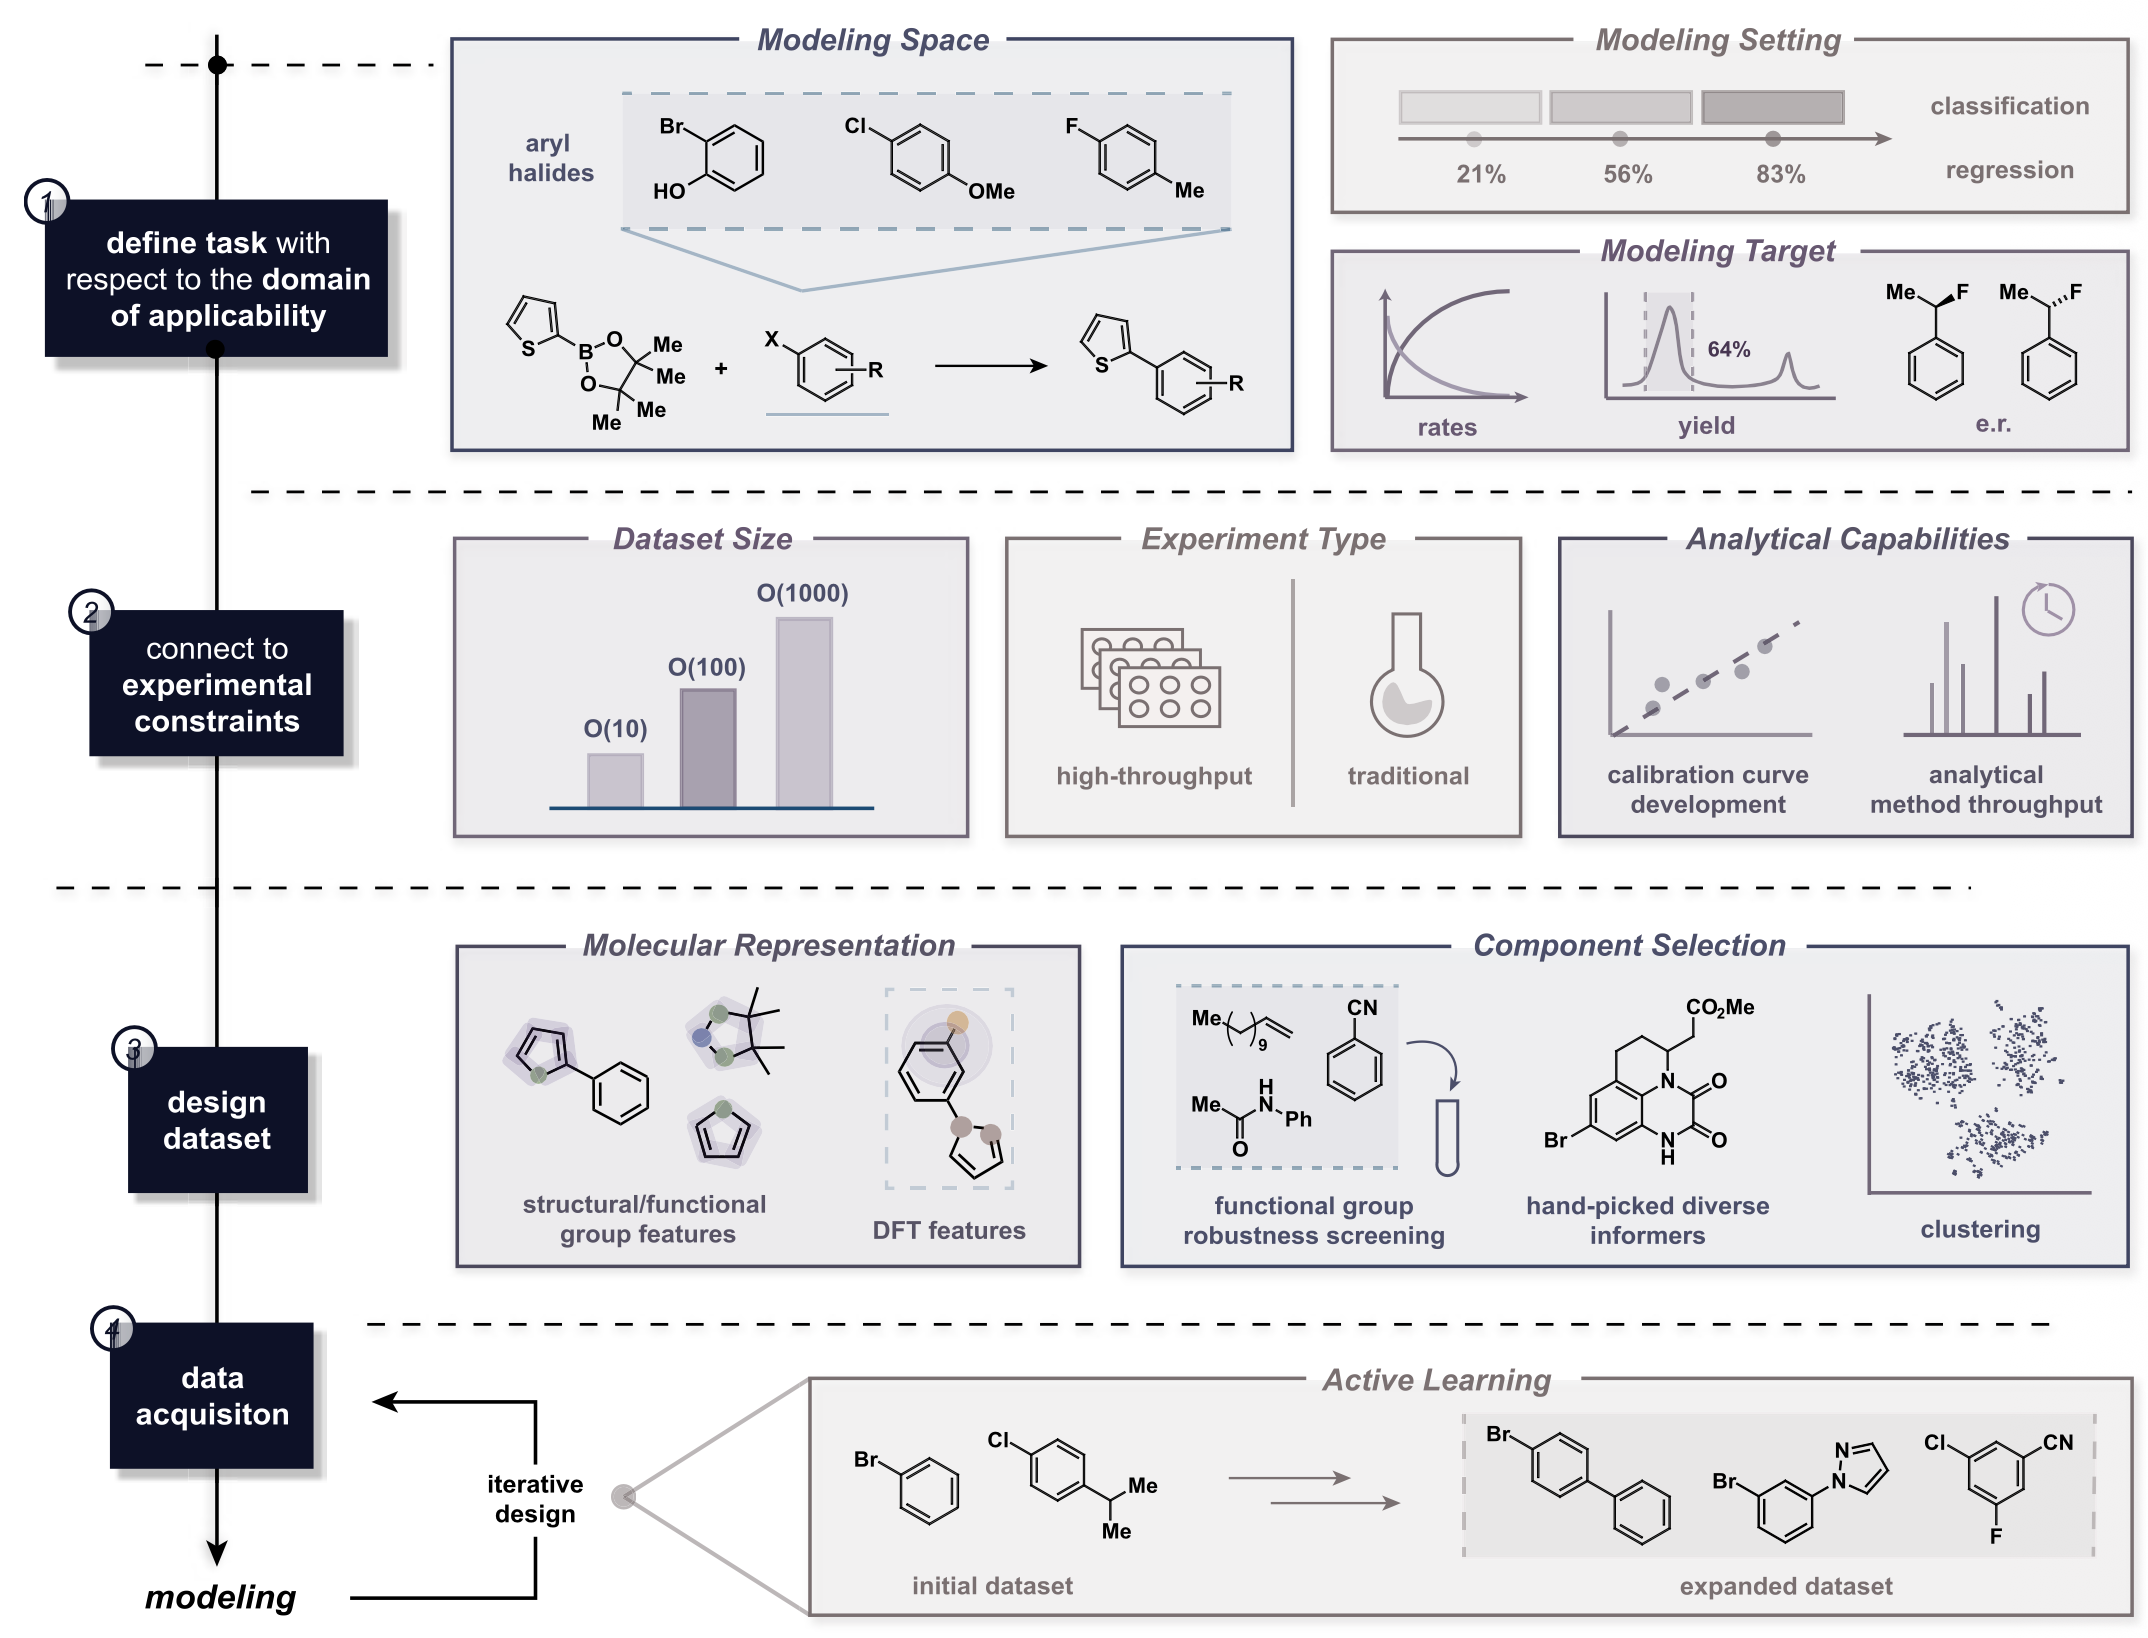
\includegraphics[width=\textwidth]{figures/CH5-dataset-design.png}
  \caption{A conceptual workflow for dataset design.}
  \label{fig5:dataset-design}
\end{figure}

The response distribution also affects the sensible modelling task.
A dataset containing a large population of inactive reactions and a smaller continuum of productive reactions may be treated as a classification problem, a regression problem, or a staged combination of both.\mcite{Haas2025}

\solution{7.0cm}{%
  \centering
  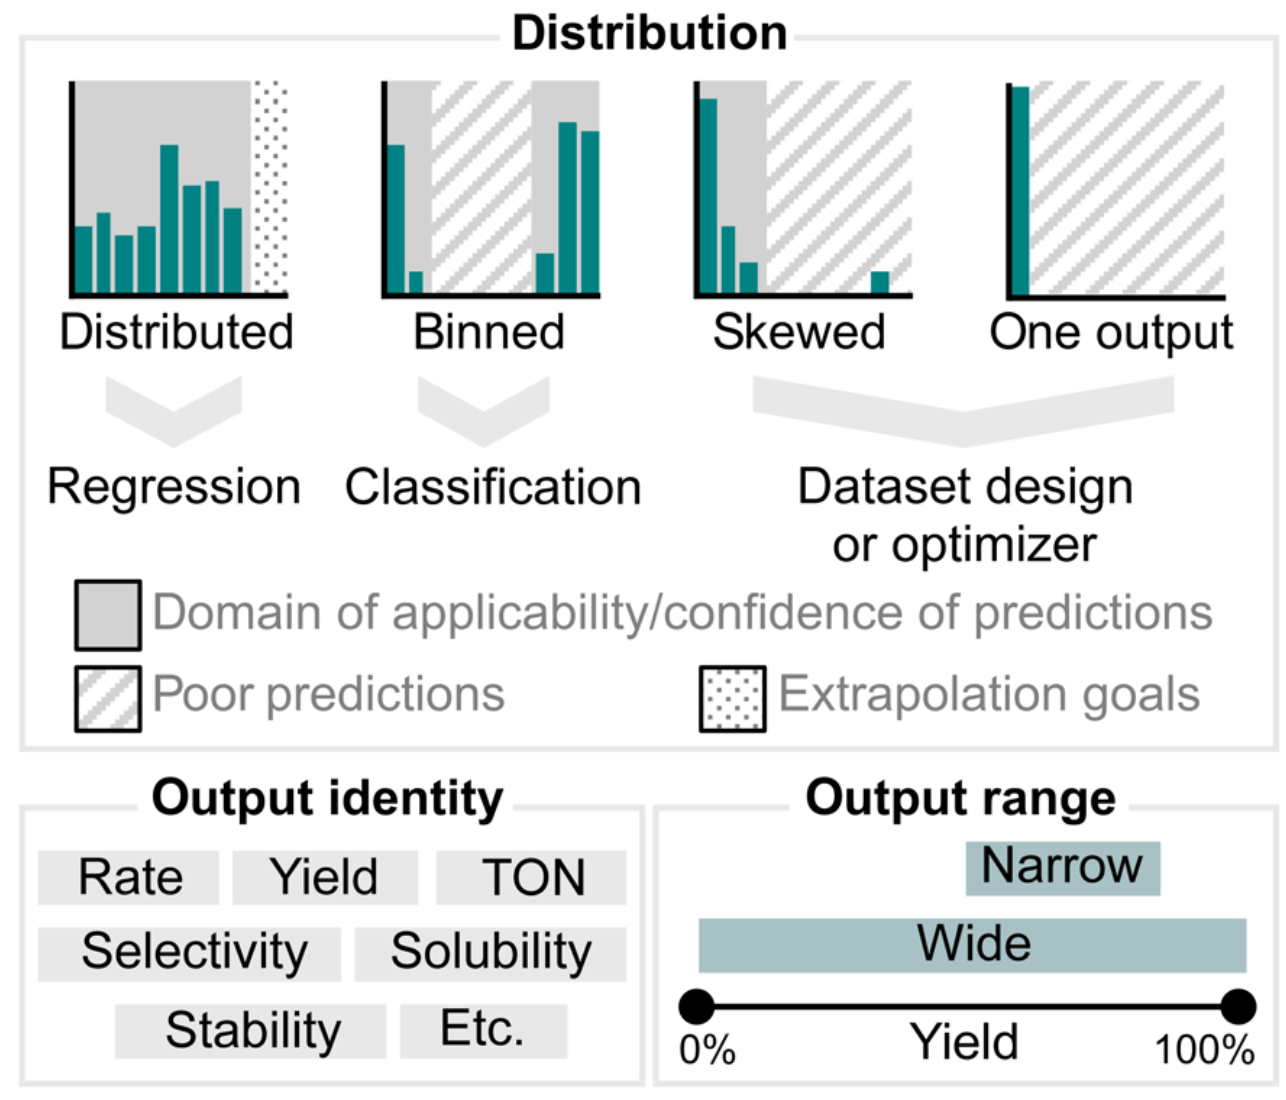
\includegraphics[width=0.5\textwidth]{figures/CH5-dataset.png}
}

\section{Reaction optimisation as modelling}

An optimisation problem begins with a decision on what the optimisation target is.
Some variables can be represented as continous numbers -- their theoretical range is infinite.
Such \keypoint{continuous variables} can include temperature, time, concentration, pressure, flow rate, and reagent equivalents.
On the other hand, \keypoint{categorical variables} can include solvent, catalyst, ligand, base, or reactor architecture.
The feasible space is smaller than the complete chemical set of all possible combinations because solubility, equipment limits, and chemical compatibility exclude some experiments.
Experimental budget and safety considerations can also drastically reduce the experimental space.

\solution{6cm}
{ \centering
  \textbf{Categorical and continuous variables}
}

The objective defines what counts as improvement.
A reaction with the highest analytical yield may not have the best isolated yield, selectivity, productivity, process mass intensity, cost, or hazard profile.
The objective function therefore encodes priorities rather than revealing a universal optimum.

\section{One variable at a time}

A common optimisation strategy in synthetic laboratories is the so-called \keypoint{one-variable-at-a-time} (OVAT) approach.
In this strategy, we change one conditions of the process while holding the others fixed.
The procedure is intuitive, produces plots that are easy to interpret locally, and can be practical when experiments are expensive or difficult to reconfigure.

A problem occurs when the effect of one variable depends on the level of another.
For example, increasing temperature may improve conversion with one base but accelerate decomposition with another.
An OVAT experiment performed at only one base identity cannot reveal the full interaction.
The resulting path can stop at a locally favourable setting while missing a better region elsewhere.

\solution{6.0cm}{%
  \centering
  \resizebox{0.7\linewidth}{!}{%
    \begin{tikzpicture}[
      axis/.style={draw=darkGrey,line width=1.4pt,->,>=Stealth},
      contour/.style={draw=darkBlue,line width=1.1pt},
      path/.style={draw=darkRed,line width=2.3pt,->,>=Stealth},
      point/.style={fill=darkRed,draw=darkRed},
      label/.style={font=\small\sffamily,text=darkGrey,align=center}
    ]
      \draw[axis] (0,0) -- (9,0) node[below] {temperature};
      \draw[axis] (0,0) -- (0,6) node[left,rotate=90] {equivalents};
      \draw[contour] (5.9,3.5) ellipse (3.0 and 2.0);
      \draw[contour] (5.9,3.5) ellipse (2.2 and 1.4);
      \draw[contour] (5.9,3.5) ellipse (1.3 and 0.8);
      \fill[darkGreen] (5.9,3.5) circle (4pt);
      \draw[path] (1.0,1.0) -- (4.2,1.0);
      \draw[path] (4.2,1.0) -- (4.2,3.1);
      \foreach \x/\y in {1.0/1.0,4.2/1.0,4.2/3.1}{\fill[point] (\x,\y) circle (3.4pt);}
      \node[label,text=darkRed] at (2.4,0.55) {OVAT path};
      \node[label,text=darkGreen] at (6.2,4.0) {true optimum};
    \end{tikzpicture}%
  }
}

\section{Design of experiments}

A framework for a factorial design where several factors are varied to estimate the curvature of the response surface is \keypoint{design-of-experiments} (DoE).
The fitted surface remains empirical, but it can identify influential variables, interactions, and promising regions more efficiently than a sequence of uncoordinated tests.

\solution{6.0cm}{%
  \centering
  \resizebox{0.45\linewidth}{!}{%
  \begin{tikzpicture}[
    axis/.style={draw=darkGrey,line width=1.4pt,->,>=Stealth},
    full/.style={fill=darkBlue,draw=darkBlue},
    centre/.style={fill=darkYellow,draw=darkGrey,line width=1pt},
    label/.style={font=\small\sffamily,text=darkGrey}
  ]
    \draw[axis] (0,0) -- (8,0) node[below] {factor A};
    \draw[axis] (0,0) -- (0,5.5) node[left,rotate=90] {factor B};
    \foreach \x in {1.2,3.7,6.2}{\foreach \y in {1.0,2.7,4.4}{\fill[full] (\x,\y) circle (3.4pt);}}
    \fill[centre] (3.7,2.7) circle (5pt);
    \node[label] at (5.8,5.0) {factorial grid};
    \node[label] at (4.9,2.25) {centre point tests curvature};
  \end{tikzpicture}%
  }
  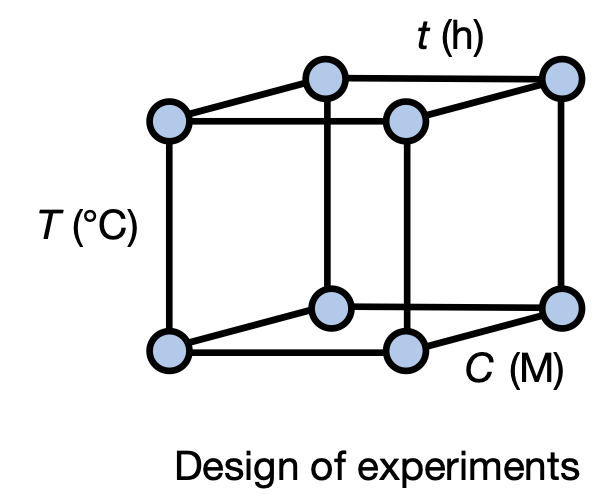
\includegraphics[width=0.45\textwidth]{figures/CH6-doe.png}
}

\section{Sequential experimentation}

A fixed design is chosen before its outcomes are known.
A sequential campaign uses each completed round to update the description of the response and to choose subsequent experiments.
This adaptivity can concentrate measurements near promising, uncertain, or chemically informative regions.

Sequential does not necessarily mean one experiment at a time.
A batch can be selected when reactions run in parallel or when instrument scheduling dominates the cost.
The price of batching is that experiments within the batch are chosen before their neighbours have returned results.
A stopping rule is also required, such as reaching a target, exhausting the budget, or observing little expected improvement.

A \keypoint{surrogate model} approximates the expensive experimental response using the observations collected so far (Fig.~\ref{fig6:bo}).
We say \textit{expensive} as it is impossible to collect data for all potential experiments.
Gaussian-process models are useful conceptually because they return both a \keypoint{mean prediction} and an \keypoint{uncertainty estimate} over the search space.
The uncertainty is generally smaller near informative observations and larger in poorly sampled regions.
This uncertainty is conditional on the chosen model and representation.
It does not guarantee that a hidden mechanism, decomposition pathway, or analytical failure has been considered.
Experimental noise, model uncertainty, and ignorance of missing chemistry should not be collapsed into one unqualified confidence interval.

\solution{10cm}{
% \begin{figure}[htbp]
  \centering
  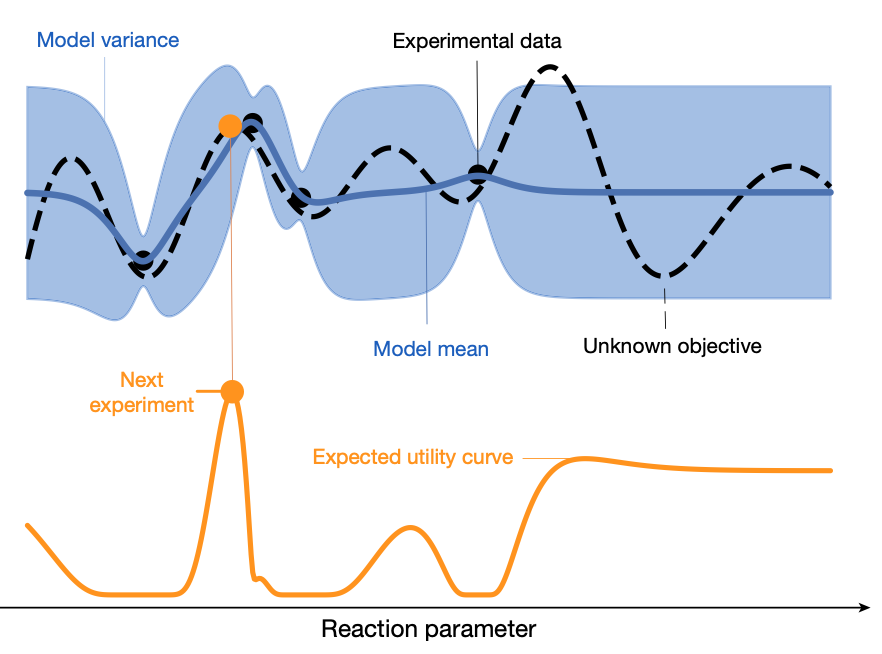
\includegraphics[width=0.8\textwidth]{figures/CH6-BO.png}
%   \caption{One-dimensional depiction of Bayesian optimisation showing a Gaussian regression surrogate model fitted to the data collected from an unknown objective. The corresponding utility function is maximised to select the next experiment.}
%   \label{fig6:bo}
% \end{figure}
}

\keypoint{Bayesian optimisation} combines a surrogate model with an \keypoint{acquisition function}.
The acquisition function ranks candidate experiments by balancing predicted performance and uncertainty.
Exploitation selects a condition expected to perform well, while exploration selects a condition that may improve the model or reveal an unsampled region.
Expected improvement is one way to combine these motives into a single ranking.

\solution{5.0cm}{%
  \centering
  \resizebox{0.94\linewidth}{!}{%
    \begin{tikzpicture}[
      candidate/.style={draw=darkBlue,fill=paleBlue,line width=1.5pt,minimum width=3.7cm,minimum height=1.0cm,align=center,font=\sffamily},
      selected/.style={draw=darkGreen,fill=paleGreen,line width=1.8pt,minimum width=3.7cm,minimum height=1.0cm,align=center,font=\sffamily},
      arrow/.style={->,>=Stealth,draw=darkGrey,line width=2pt},
      label/.style={font=\small\sffamily,text=darkGrey,align=center}
    ]
      \node[candidate] (mean) at (0,1.4) {high predicted value\\low uncertainty};
      \node[candidate] (unc) at (0,-1.4) {moderate predicted value\\high uncertainty};
      \node[candidate] (acq) at (6,0) {acquisition function};
      \node[selected] (next) at (12,0) {next experiment};
      \draw[arrow] (mean) -- (acq);
      \draw[arrow] (unc) -- (acq);
      \draw[arrow] (acq) -- (next);
      \node[label] at (6,-1.4) {balance exploitation and exploration};
    \end{tikzpicture}%
  }
}

Shields and co-workers benchmarked Bayesian reaction optimisation across several reaction datasets and compared machine recommendations with human decisions (Fig.~\ref{fig6:bo-human}).\mcite{Shields2021}
In their `game', participants had one month to find optimal reaction conditions while performing five reactions per day (the `strive for five' synthetic chemistry mentality).
A web application returned the experimental results to the participants based on the outcomes of a previous high-throughput experimental campaign.
A method that repeatedly reaches good regions with fewer experiments is more generally useful than one that occasionally finds an excellent point by chance.
Researchers have since applied this approach to many other reaction optimisation projects.

\begin{figure}[htbp]
  \centering
  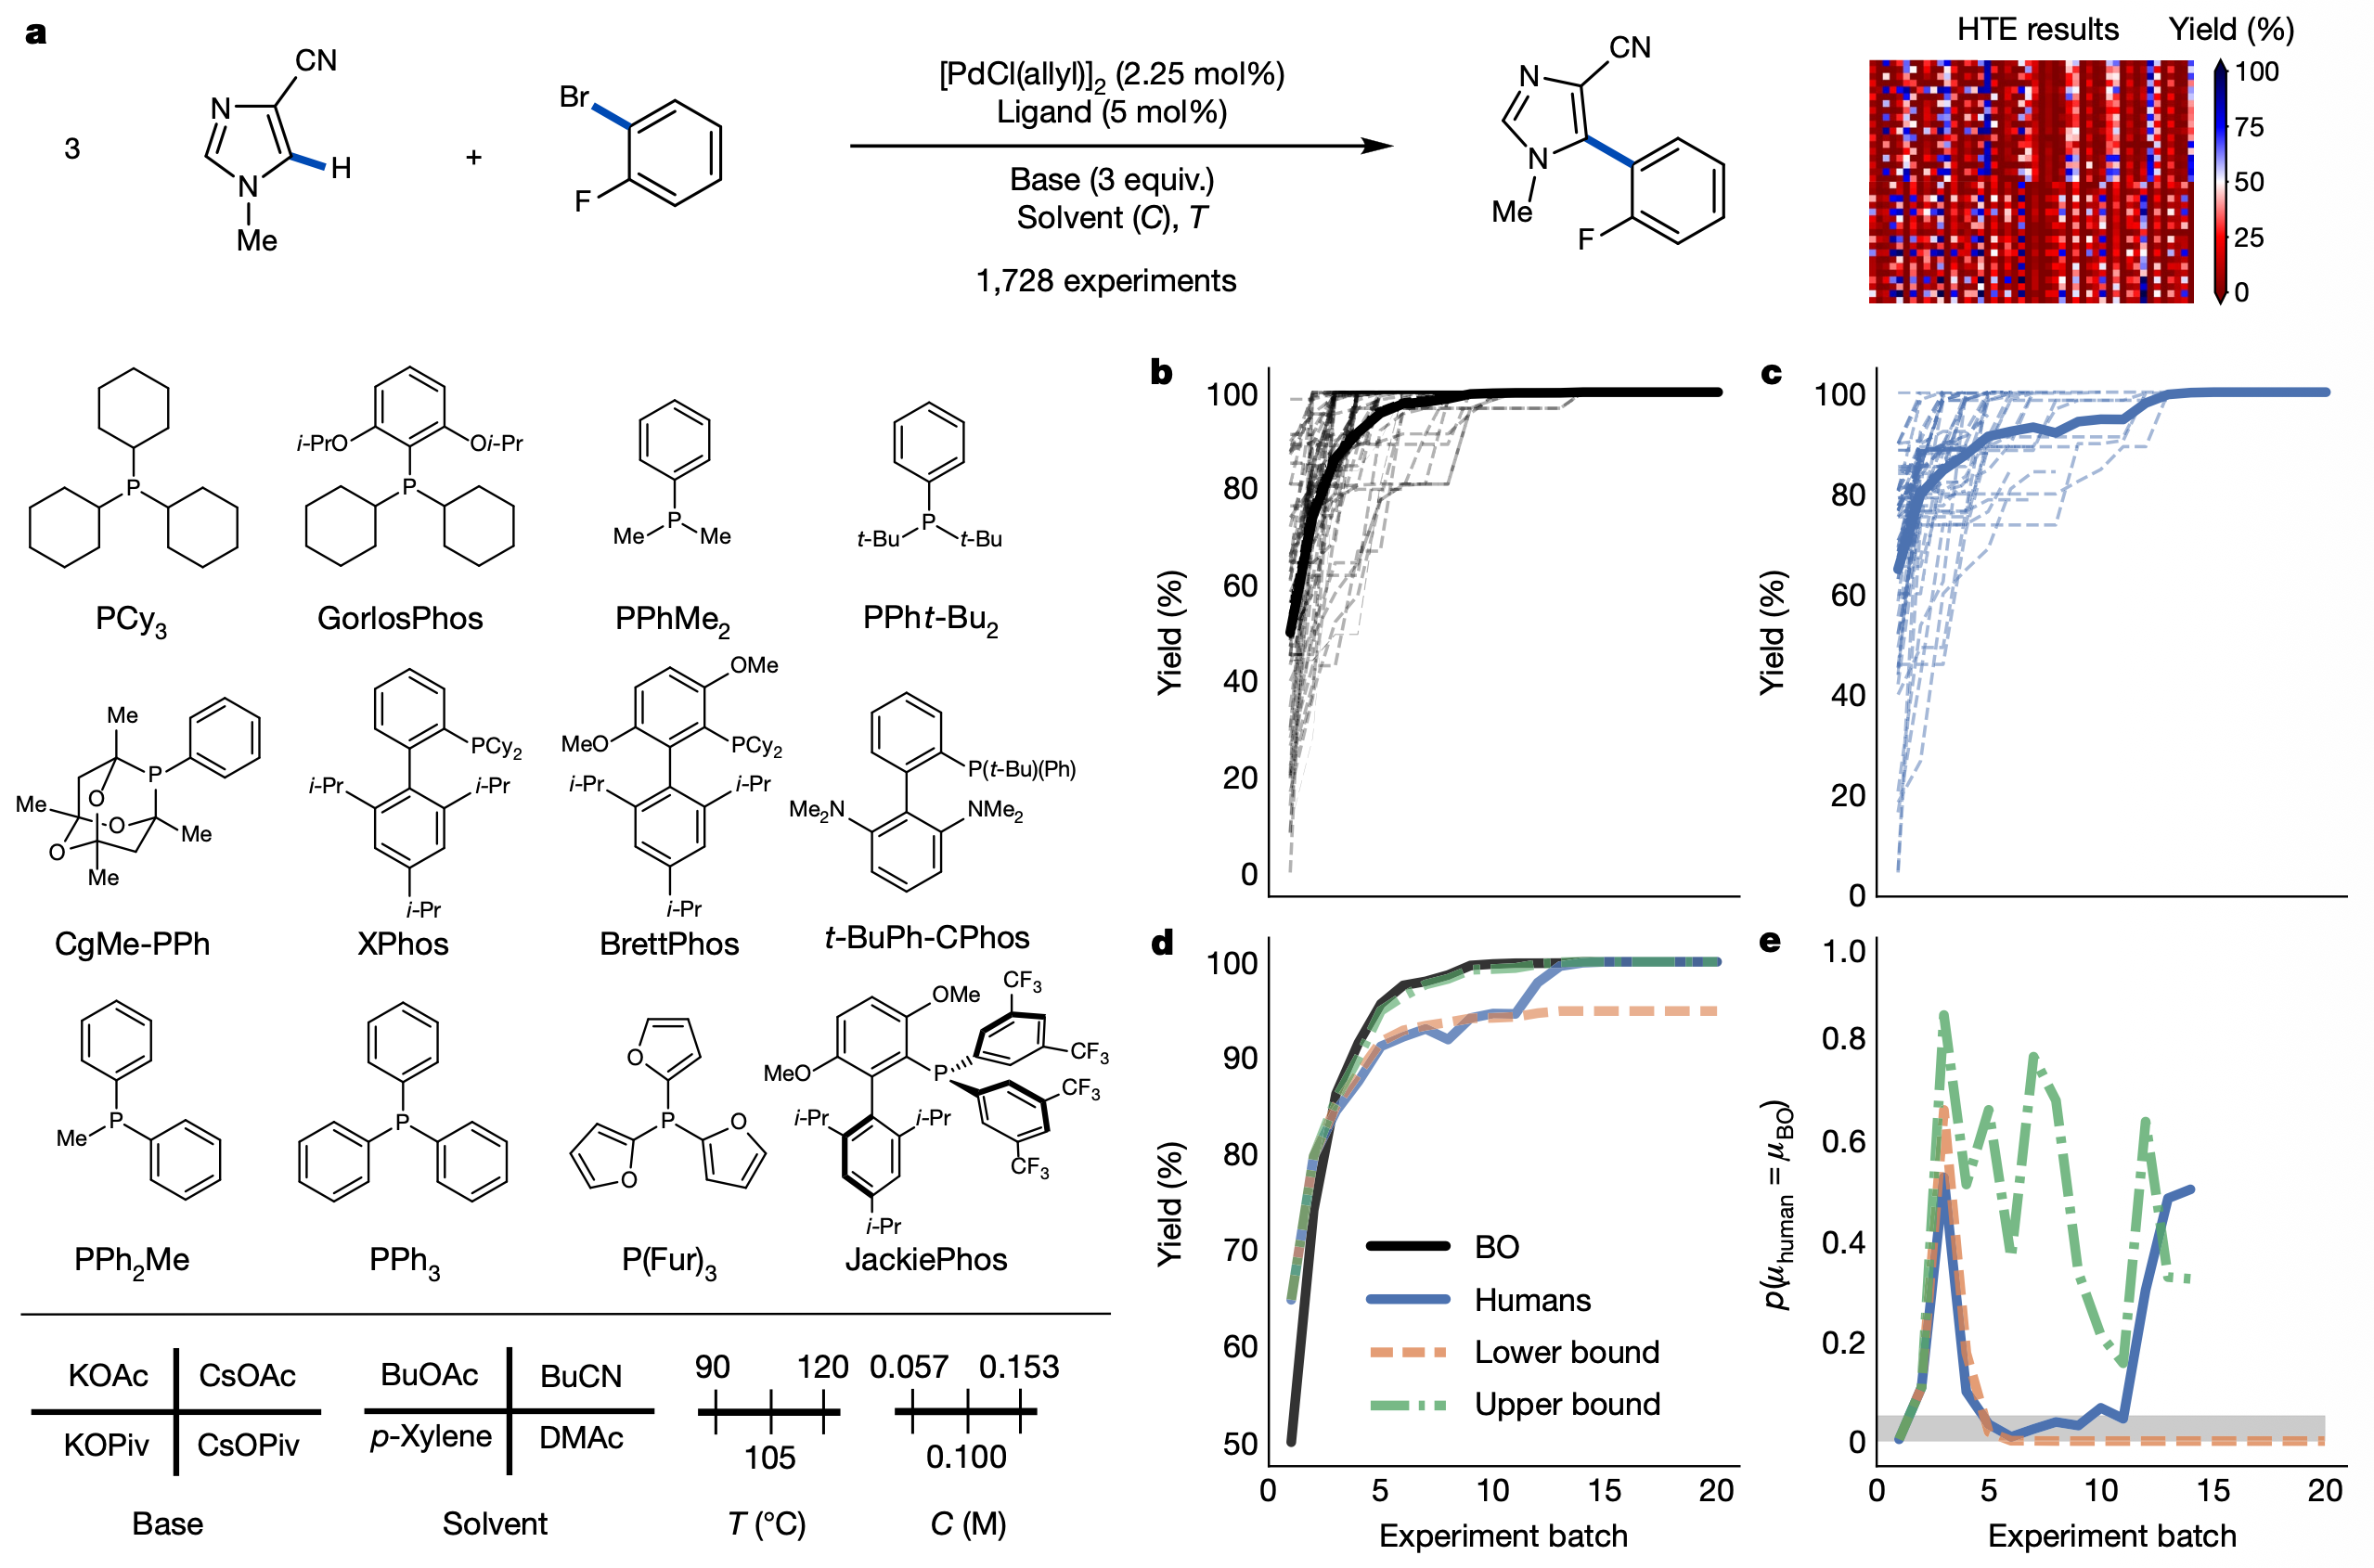
\includegraphics[width=\textwidth]{figures/CH6-BOvsDoyle.png}
  \caption{Comparison of a Bayesian optimisation performance against human researchers with fixed experimental budget.}
  \label{fig6:bo-human}
\end{figure}

\section{Multiple objectives and constraints}

Chemical optimisation often has several objectives.
Yield and selectivity may conflict with productivity, solvent use, energy demand, cost, or hazard.
A solution is dominated when another tested or predicted solution is at least as good in every objective and better in at least one.
The non-dominated solutions form a \keypoint{Pareto front}.
The Pareto front does not choose among the trade-offs.
It exposes the consequences of prioritising one objective over another.
A chemist or process team must still decide whether a small gain in yield justifies additional waste, cost, or risk.
Unsafe or technically impossible regions should be represented as constraints rather than rewarded merely because the model is uncertain there.

\solution{7.0cm}{%
  \centering
  \resizebox{0.86\linewidth}{!}{%
    \begin{tikzpicture}[
      axis/.style={draw=darkGrey,line width=1.4pt,->,>=Stealth},
      dominated/.style={fill=darkGrey,draw=darkGrey},
      pareto/.style={fill=darkGreen,draw=darkGreen},
      frontier/.style={draw=darkGreen,line width=2.2pt},
      unsafe/.style={fill=paleRed,draw=darkRed,opacity=0.55},
      label/.style={font=\small\sffamily,text=darkGrey,align=center}
    ]
      \draw[axis] (0,0) -- (9.5,0) node[below] {yield $\rightarrow$};
      \draw[axis] (0,0) -- (0,6) node[left,rotate=90] {selectivity $\rightarrow$};
      \foreach \x/\y in {1.2/1.2,2.1/2.0,2.8/1.3,3.6/2.7,4.5/2.0,5.1/3.2,6.1/2.8}{\fill[dominated] (\x,\y) circle (3.2pt);}
      \foreach \x/\y in {2.0/4.9,3.5/4.6,4.9/4.1,6.2/3.6,7.2/3.0}{\fill[pareto] (\x,\y) circle (4pt);}
      \draw[frontier] plot[smooth] coordinates {(2.0,4.9) (3.5,4.6) (4.9,4.1) (6.2,3.6) (7.2,3.0)};
      \node[label,text=darkGreen] at (4.8,5.2) {Pareto front};
    \end{tikzpicture}%
  }
}

\section{Predicting catalyst selectivity}

Zahrt and co-workers began from a large in-silico library of synthetically accessible chiral phosphoric-acid catalysts (Fig.~\ref{fig5:denmark-summary}).\mcite{Zahrt2019}
They calculated conformer-aware average steric occupancy descriptors and selected a representative "universal training set" from the resulting catalyst space.
The training set was therefore designed to cover the wider chemical space rather than assembled only from familiar catalysts, allowing for subsequent interpolation within the representation.

\begin{figure}[htbp]
  \centering
  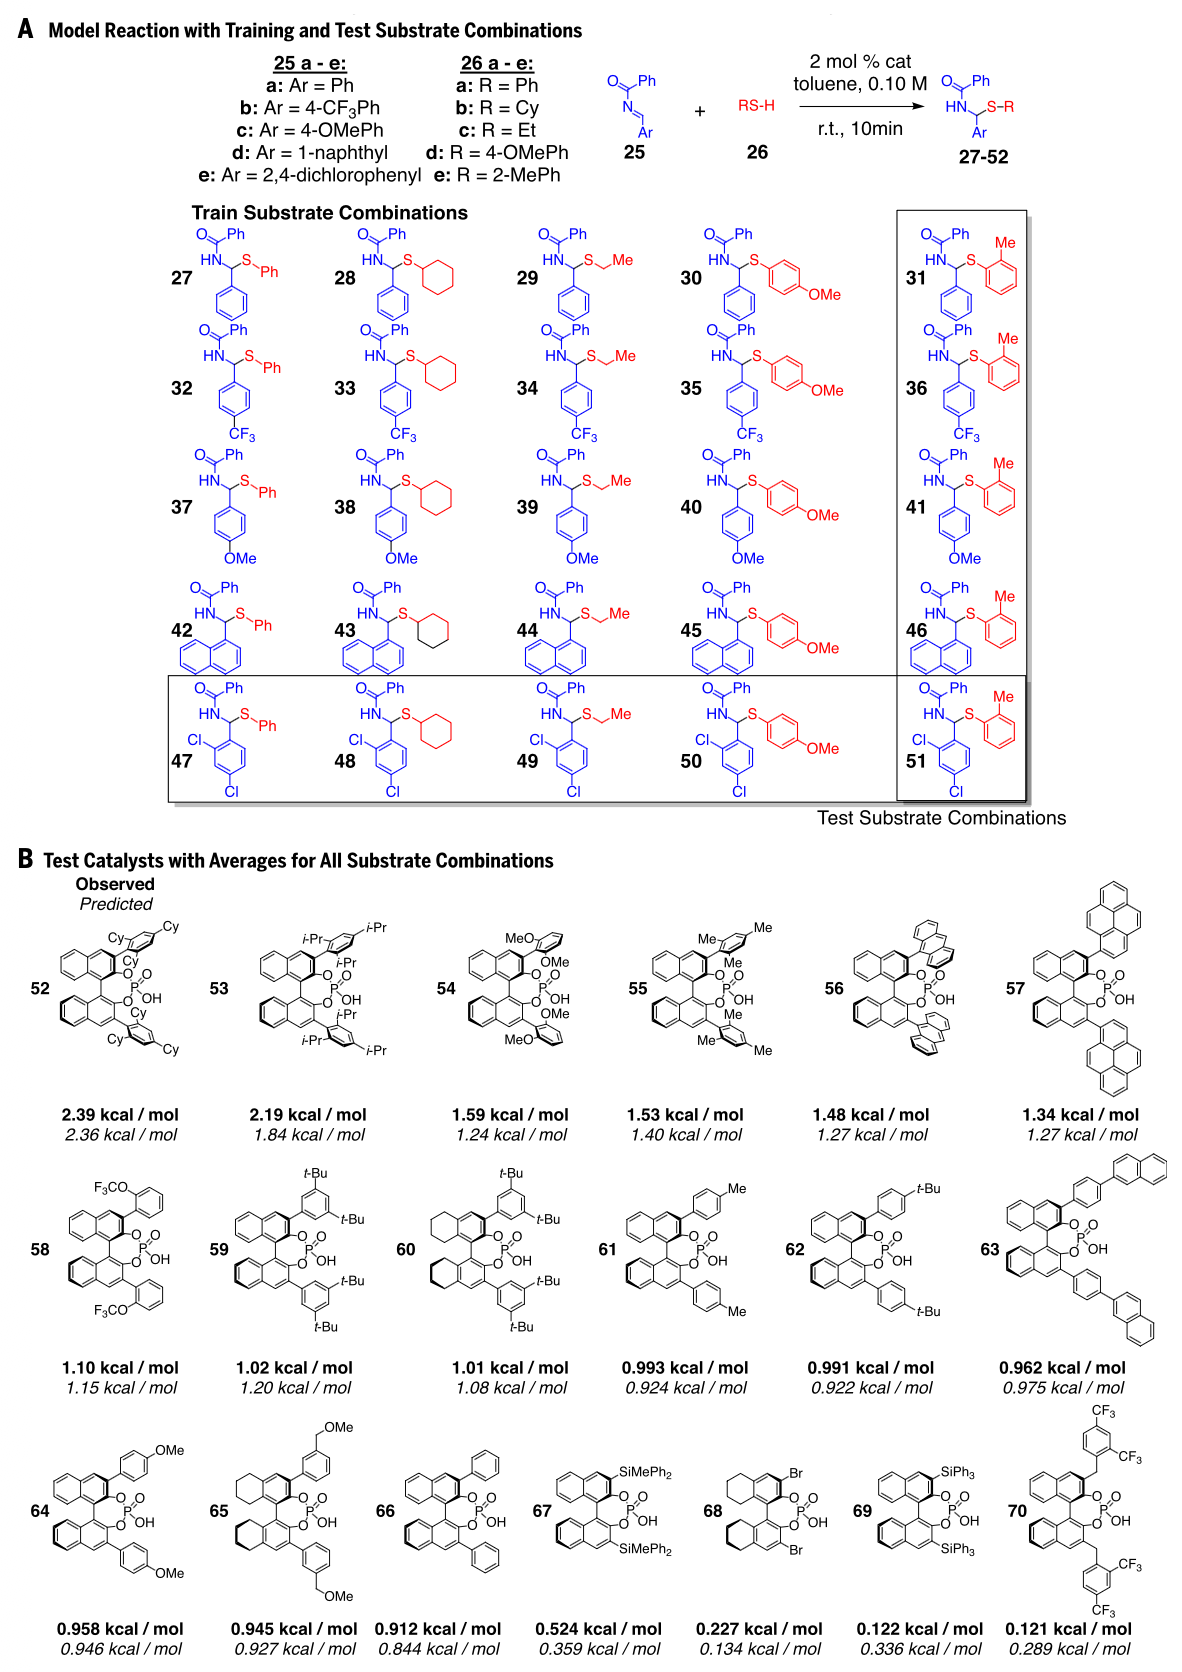
\includegraphics[width=\textwidth]{figures/CH5-denmark2.png}
  \caption{Experimental workflow to measure average selectivity for each of the 43 catalysts in the "universal training set". All substrate combinations were tested against the same set of catalysts.}
  \label{fig5:denmark-exp}
\end{figure}

\begin{figure}[htbp]
  \centering
  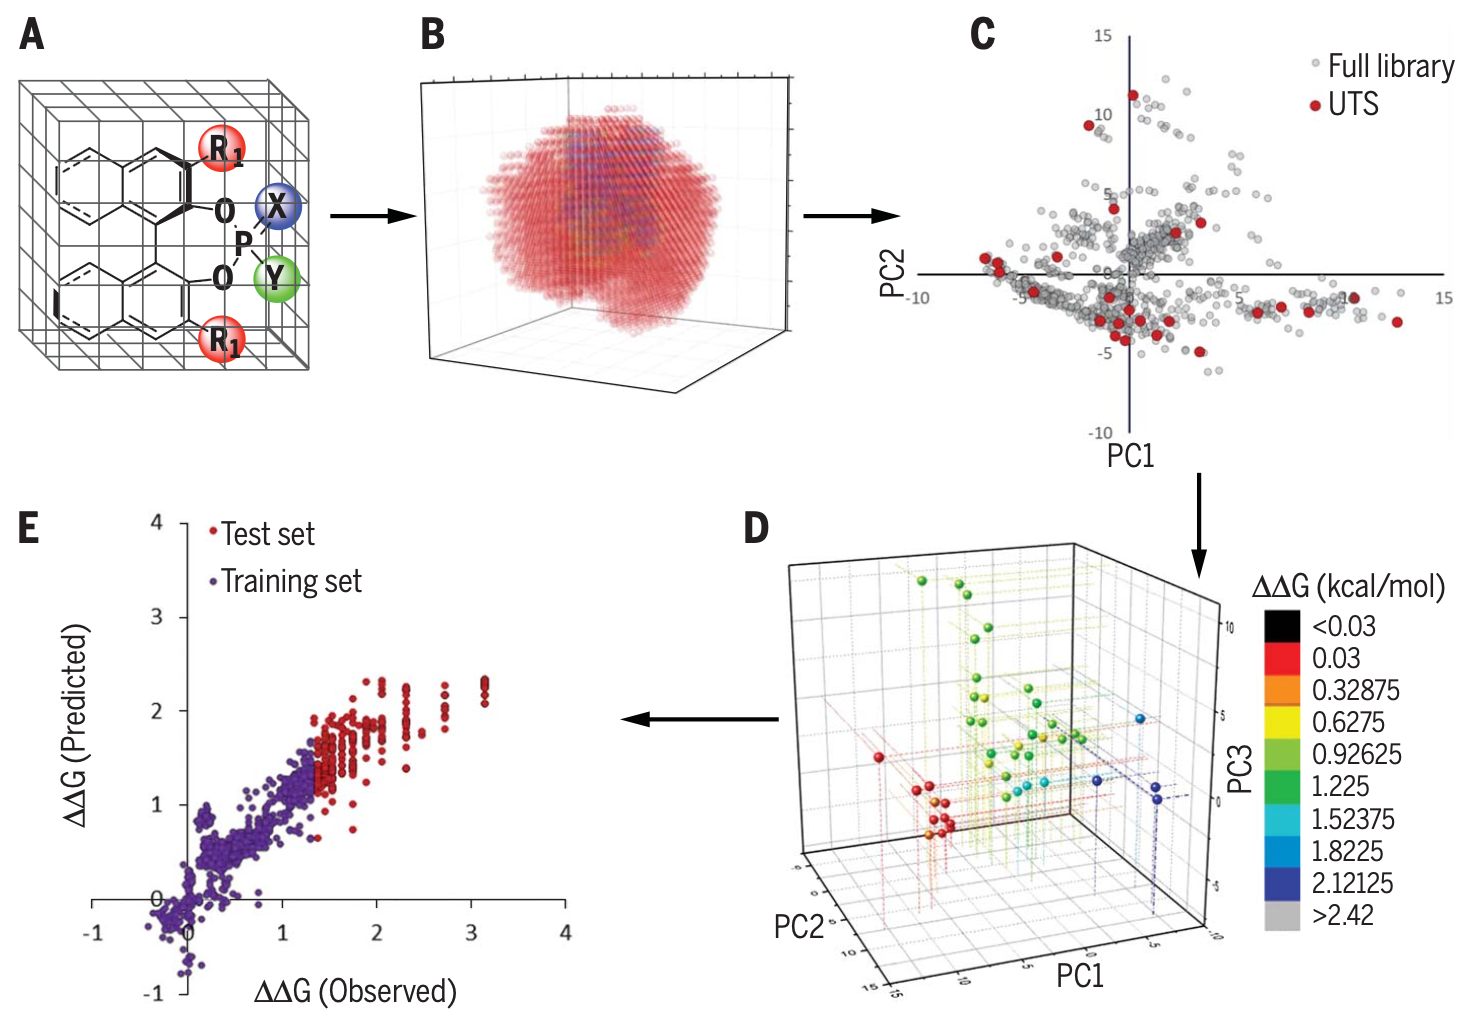
\includegraphics[width=\textwidth]{figures/CH5-denmark.png}
  \caption{Summary of the cheminformatics workflow from \textit{Zahrt et al.}. \textbf{A.} Generation of a large virtual library of catalyst candidates. \textbf{B.} Calculation of descriptors. \textbf{C.} Selection of a training set. \textbf{D.} Acquisition of experimental selectivity data. \textbf{E.} Validation of training on low- and moderately-selective reactions to predict high selectivity reactions.}
  \label{fig5:denmark-summary}
\end{figure}

The authors then performed 2150 experiments ($43 \text{ catalysts} \times 25\,\mathrm{products} \times 2\,\mathrm{repeats}$) and measured average selectivity for each catalyst across a range of substrates (Fig.~\ref{fig5:denmark-exp}).
They have then applied the resulting model to the entire catalyst space, which allowed them to \keypoint{identify the best performing phosphoric acid catalyst for the reaction}.
Importantly, their predictions were validated experimentally.
The authors also tested whether training the model just on reactions resulting in low and medium selectivity would be able to predict highly performing catalysts.
Their approach performed surprisingly well for such generalisation, implying that extrapolation within the response (while keeping within the representation) is feasible.

Interestingly, the sterics descriptor developed by Zahrt \textit{et al.} (the Average Steric Occupancy, \textbf{ASO}) included data obtained from the catalyst's conformer population.
This concept of treating our dependent variables as entire conformer ensemble properties rather than static molecules is crucial in the coming example of cross-coupling reactivity cliffs.

\section{Interpretative reaction modelling}

\begin{figure}[htbp]
  \centering
  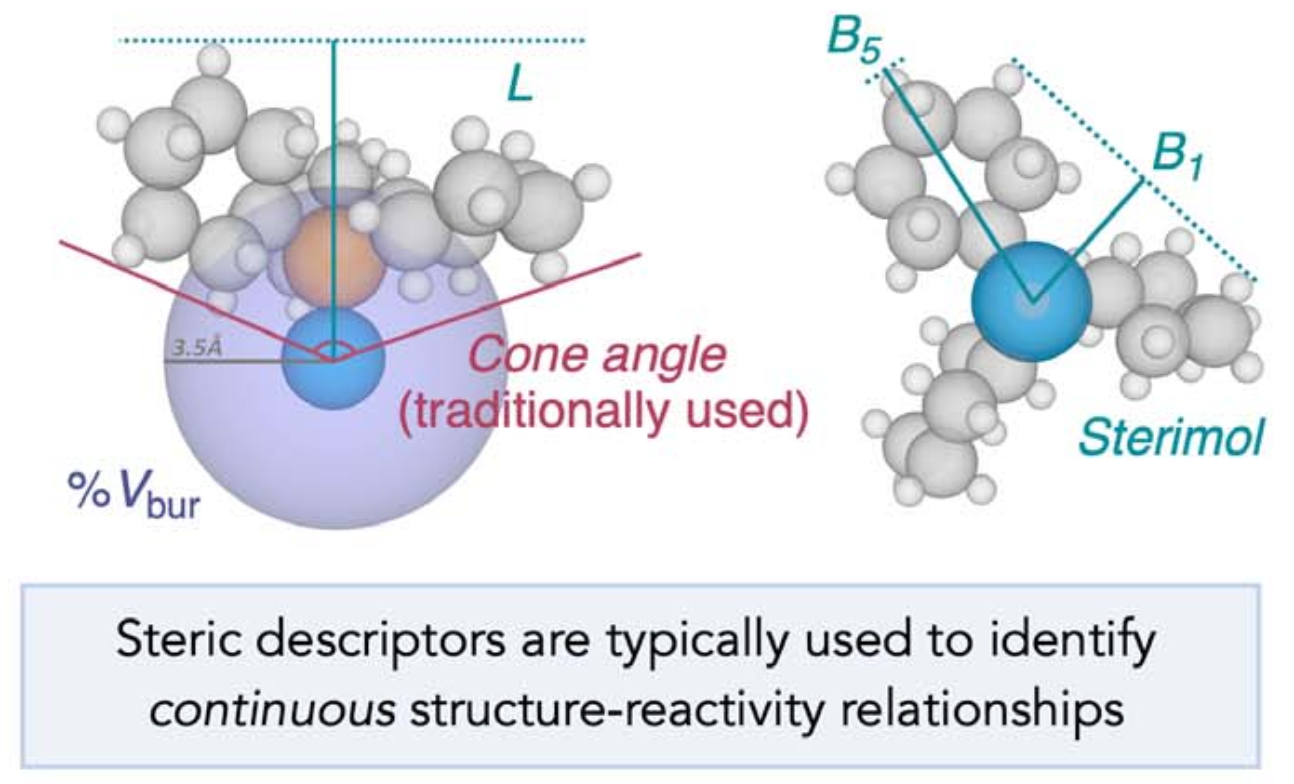
\includegraphics[width=0.34\textwidth]{figures/CH5-vbur-1.png}
  \vspace{3em}
  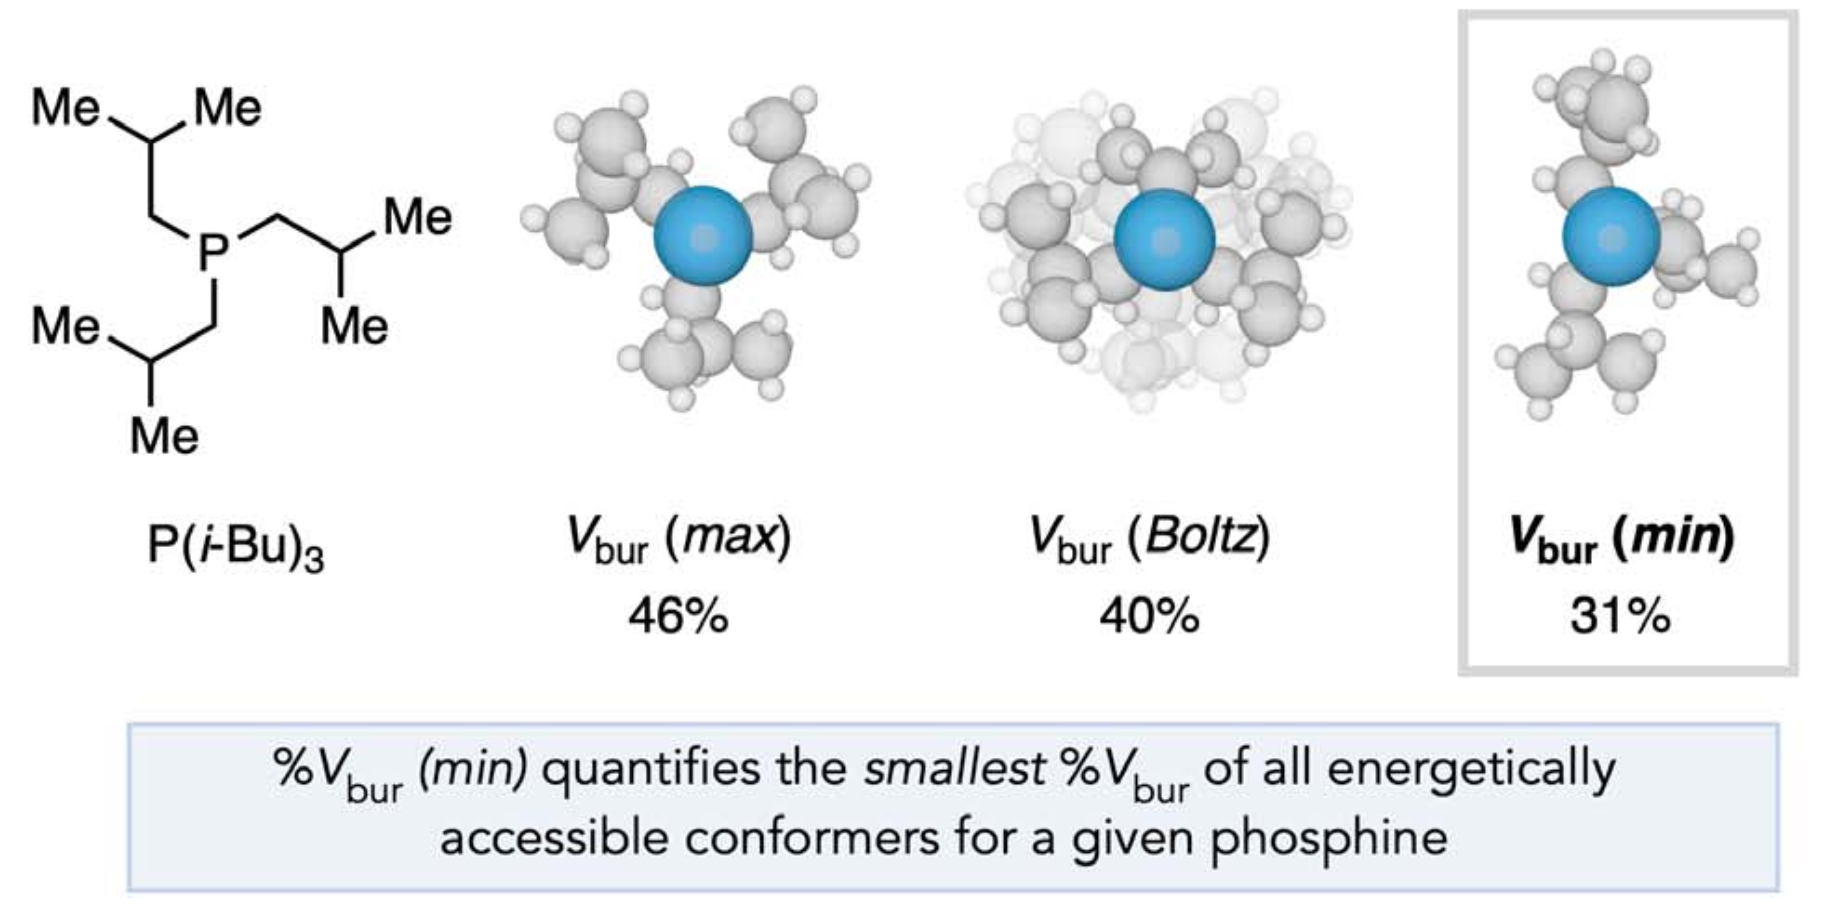
\includegraphics[width=0.64\textwidth]{figures/CH5-vbur-2.png}
  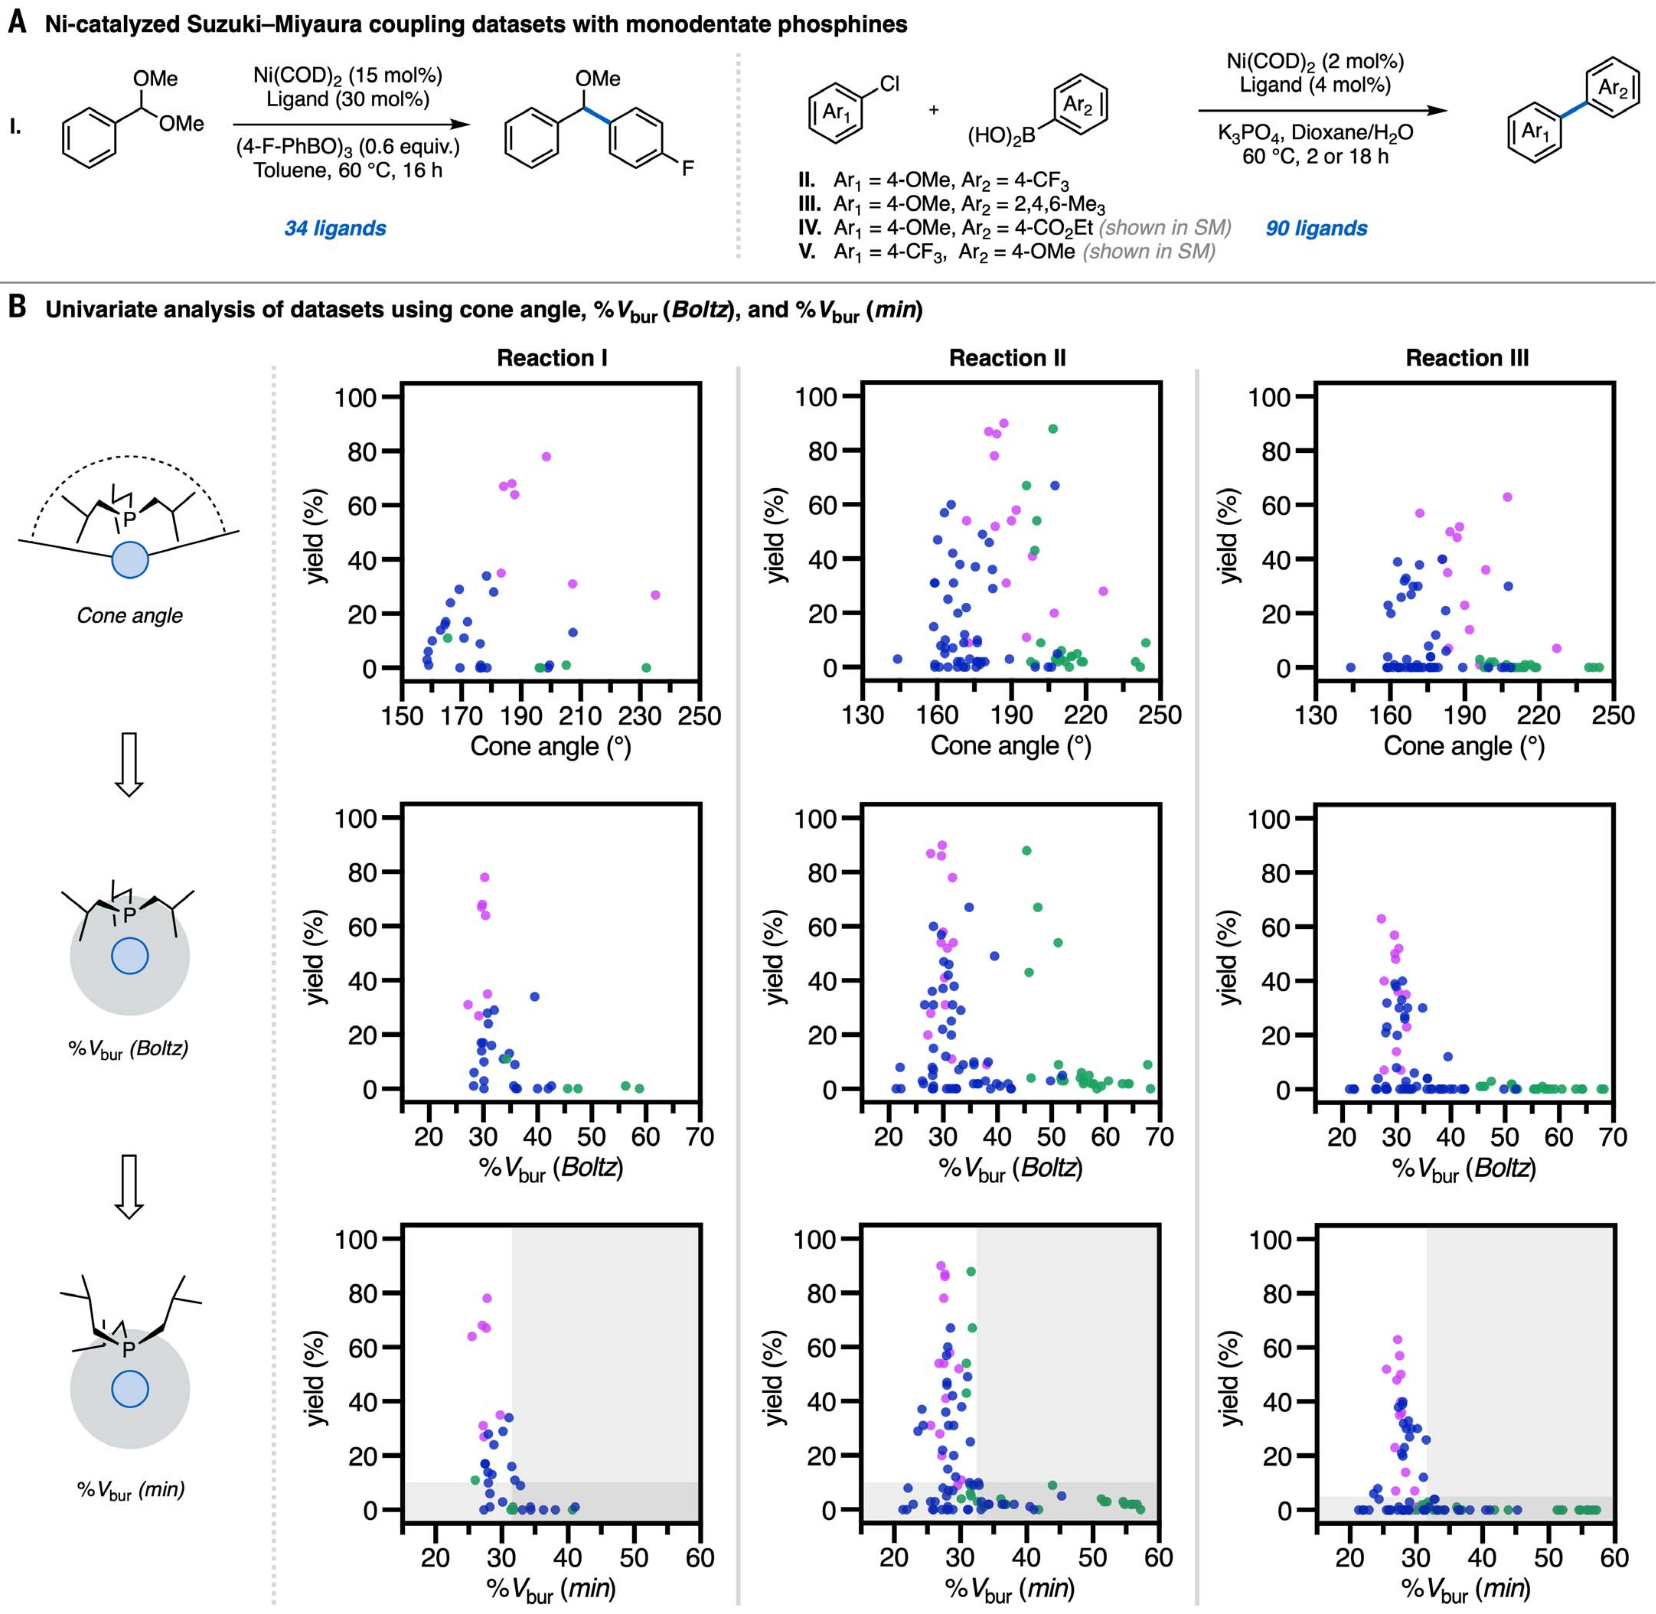
\includegraphics[width=\textwidth]{figures/CH5-cliffs.png}
  \caption{(Top) Steric descriptors for a conformer ensemble of phosphine ligands. (Bottom) Reactivity cliffs observed for steric descriptors in nickel-catalysed cross-coupling reactions. Minimum buried volume separated active and inactive ligand regimes close to a threshold, and was related to ligation state at nickel.}
  \label{fig5:cliff}
\end{figure}

Newman-Stonebraker and co-workers combined data from nickel- and palladium-catalysed cross-coupling reactions with descriptors from the \textit{kraken} phosphine library (Fig.~\ref{fig5:cliff}).\mcite{NewmanStonebraker2021}
They chose ultiple linear regression as the underlying model, as its mathematical form is transparent and the descriptors can be chemically motivated.
However, if two descriptors carry nearly the same information, their fitted coefficients may be unstable even when the combined predictions remain satisfactory.
Scaling, descriptor selection, repeated fitting, and inspection of correlations are therefore part of chemical interpretation rather than optional preprocessing.
A smooth model assumes that similar inputs tend to produce similar responses.
Reactivity cliffs violate that expectation because a small change in representation is associated with a large change in chemical outcome.
Such cliffs can expose a boundary between catalytic states or mechanisms that is compressed into one descriptor space.

\begin{warningbox}
  A sharp statistical boundary should prompt a chemical question.
  It should not be labelled as a mechanistic boundary until independent evidence supports that interpretation.
\end{warningbox}

The authors investigated a number of different steric parameters related to \keypoint{minimum energy conformations}, \keypoint{smallest parameters values across the ensemble}, as well as \keypoint{Boltzmann-averaged parameters}.
Minimum buried volume separated active and inactive ligand regimes close to a threshold, whereas cone angle did not provide the same useful classification (Fig.~\ref{fig5:cliff}).
\keypoint{Spectroscopic studies then connected the descriptor boundary to phosphine ligation state at nickel.}
Minimum buried volume boundary was directly related to one or two molecules of the phosphine ligand coordinating the nickel centre.
The case is powerful because the statistical separation is supported by an experimentally testable chemical interpretation.

\begin{warningbox}
  \keypoint{Feature importance is not automatically mechanistic importance.}
\end{warningbox}

\section{Testing the models}

A fitted model must be tested on data that were not used to determine its parameters.
A random row split is useful only when the intended future prediction resembles another random row from the same population.
If the scientific question concerns a new substrate family, catalyst scaffold, or reagent class, then the corresponding component should be held out during validation.

\begin{insightbox}
  \keypoint{How to select a test set?}
   A good test set does not include molecules that were used for training, otherwise it will not correctly assess the performance. However, often when looking at reactions datasets, a random split of reactions into training and test sets might implicitly contain all reagent combinations that were actually used to develop a model.
\end{insightbox}

Residuals are the differences between observed and predicted responses.
Small, unstructured residuals are consistent with a model capturing the dominant relationship over the sampled domain.
A group of residuals associated with one substrate class, catalyst family, or condition range can instead indicate a missing descriptor, a measurement problem, or a change in chemical regime.

\solution{5.0cm}{%
  \centering
  \resizebox{0.6\linewidth}{!}{%
    \begin{tikzpicture}[
      axis/.style={draw=darkGrey,line width=1.4pt,->,>=Stealth},
      datum/.style={fill=darkBlue,draw=darkBlue},
      outlier/.style={fill=darkRed,draw=darkRed},
      fit/.style={draw=darkGreen,line width=2.2pt},
      residual/.style={draw=darkRed,dashed,line width=1.6pt,<->,>=Stealth},
      label/.style={font=\small\sffamily,text=darkGrey,align=center}
    ]
      \draw[axis] (0,0) -- (8,0);
      \draw[axis] (0,0) -- (0,6);
      \draw[fit] (0.5,0.5) -- (7.3,5.7);
      \foreach \x/\y in {1.0/0.9,1.8/1.6,2.6/2.3,3.5/3.0,4.4/3.7,5.2/4.4,6.2/5.0}{\fill[datum] (\x,\y) circle (3pt);}
      \fill[outlier] (5.7,2.0) circle (4pt);
      \draw[residual] (5.7,2.0) -- (5.7,4.55);
      \node[label,text=darkRed,anchor=west] at (5.9,3.2) {error, missing variable,\\or new chemical regime?};
    \end{tikzpicture}%
  }
}

\section{Model and representation choice}

Kalikadien, Valsecchi and co-workers generated 3552 measurements for rhodium-catalysed asymmetric hydrogenation across catalyst, substrate, solvent, pressure, temperature, and time choices.\mcite{Kalikadien2024}
They evaluated the effect of those variables on hydrogenation conversion and enantiomeric excess (Fig.~\ref{fig5:pidko1}).
A subset of 960 of those reactions was subsequently used for ML modelling to predict reactivity.
The conversion displayed a binary distribution (hence suitable for a classification task), while the enantiomeric excess was more normally distrubuted (hence a regression task).

\begin{figure}[htbp]
  \centering
  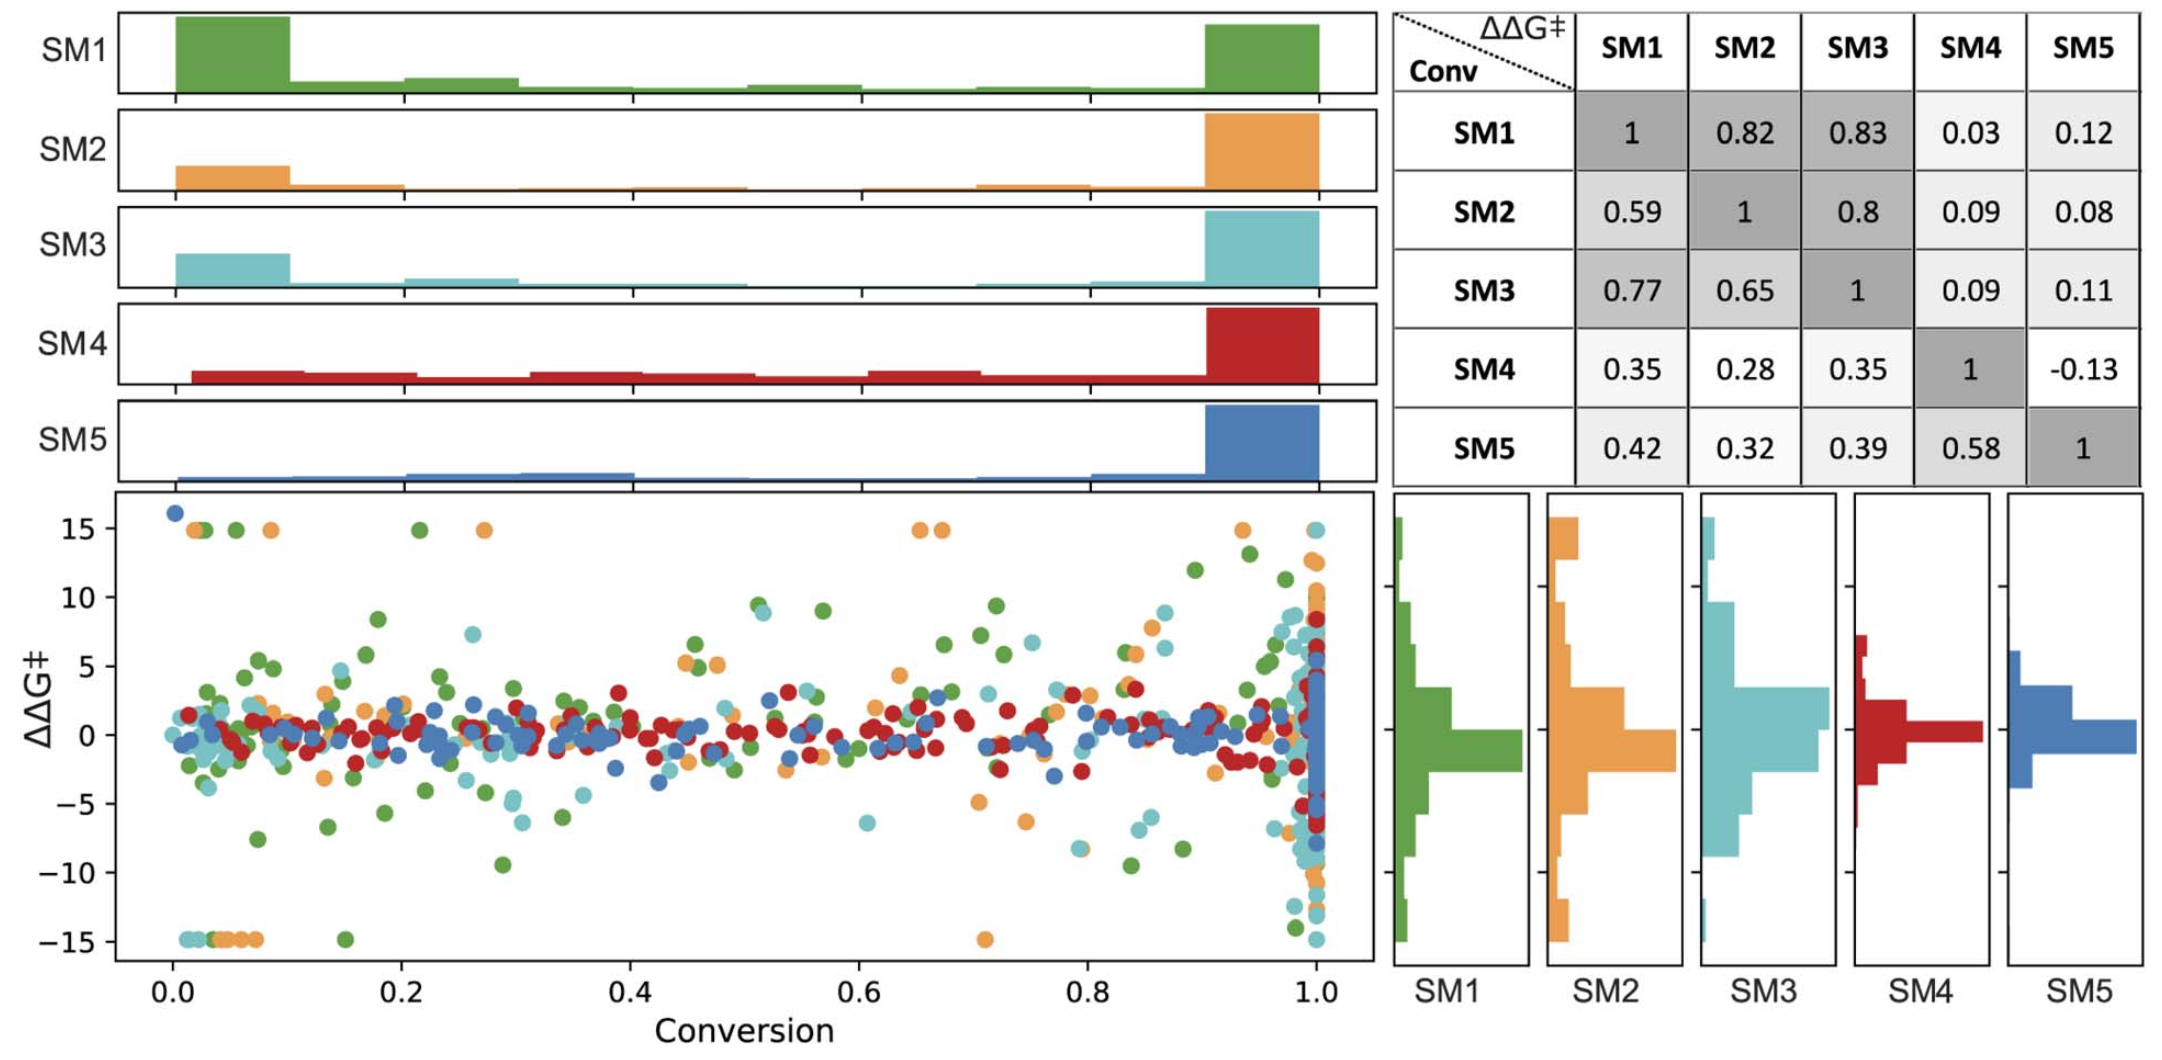
\includegraphics[width=\textwidth]{figures/CH5-pidko1.png}

  \caption{Distribution of conversion and enantioselectivity observed for the five different substrates studied by Kalikadien, Valsecchi \textit{et al.}.}
  \label{fig5:pidko1}
\end{figure}

\begin{figure}[htbp]
  \centering
  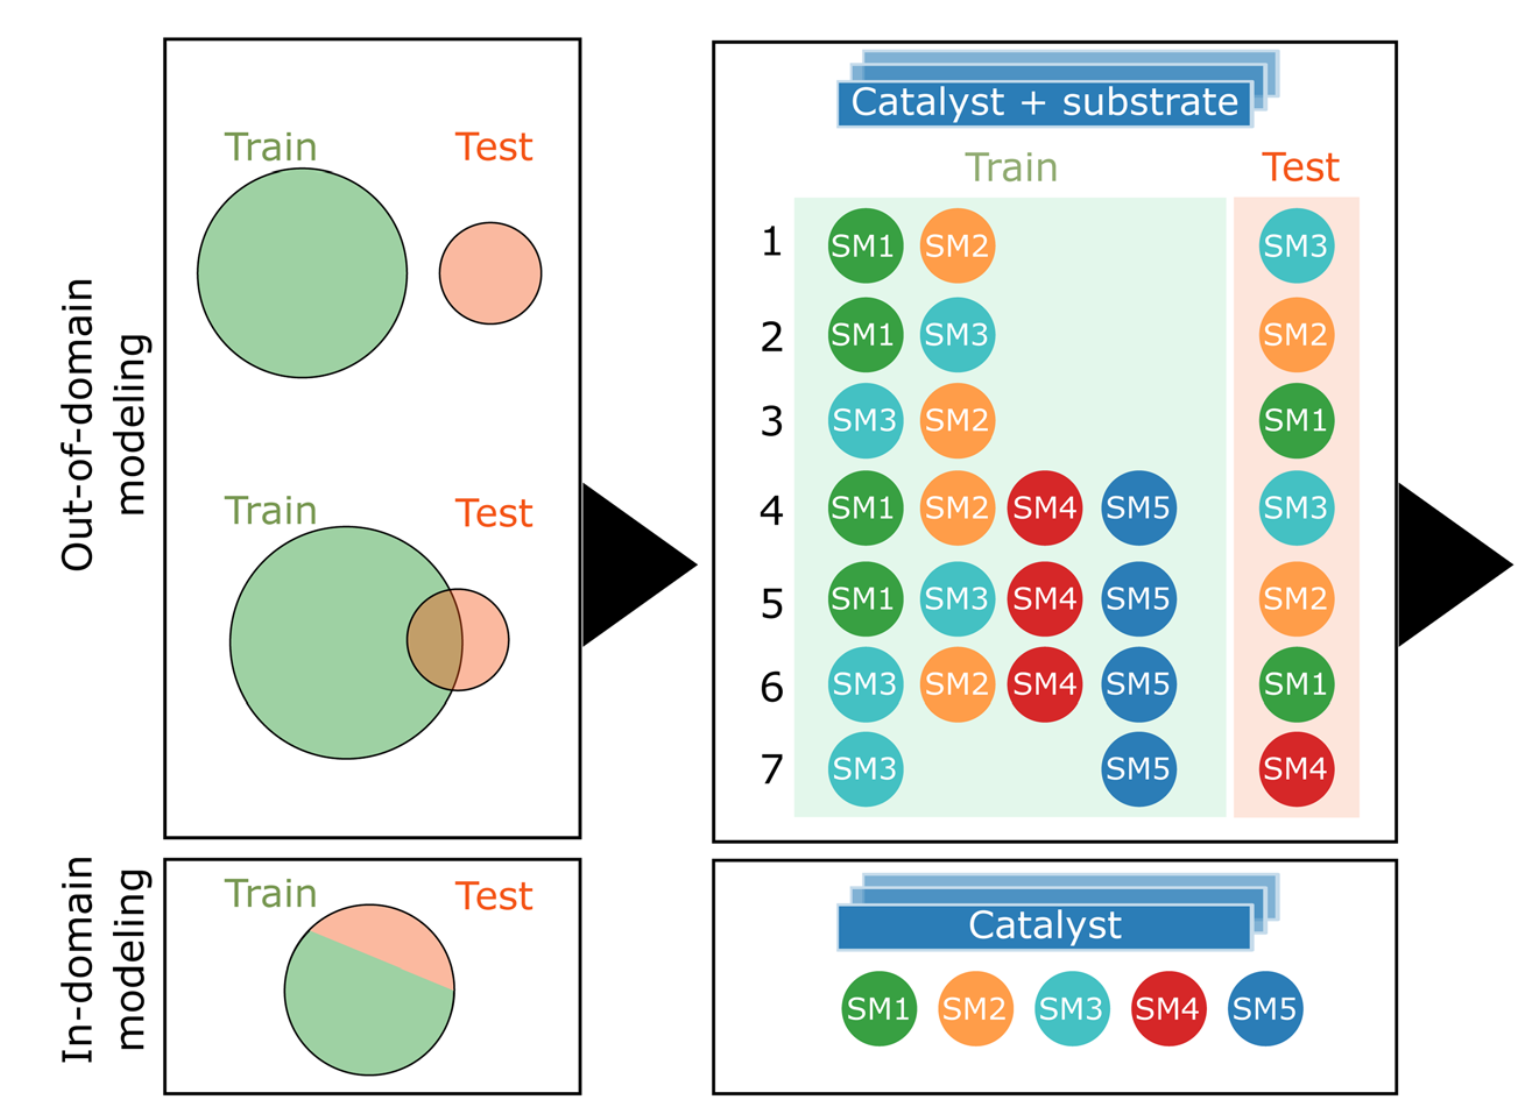
\includegraphics[width=0.6\textwidth]{figures/CH5-pidko2.png}

  \caption{Design of the in-domain and out-of domain ML workflows.}
  \label{fig5:pidko2}
\end{figure}

The authors set out to see if a model trained on unrelated substrates (out-of-domain) could be used to accurately predict the conversion and selectivity for target substrates (Fig.~\ref{fig5:pidko2}).
This approach is contrasted with merely selecting a random subset of reaction data for model training (in-domain).
The out-of-domain results demonstrated comparable performance for a range of different molecular descriptors, indicating that the models were not able to capture the chemistry and performance relied solely on ligand differentiation (Fig.~\ref{fig5:pidko3}). 
The in-domain results suggested that for this system simple features (\textit{e.g.,} fingerprints) performed as well as DFT-level descriptors.

\begin{figure}[htbp]
  \centering
  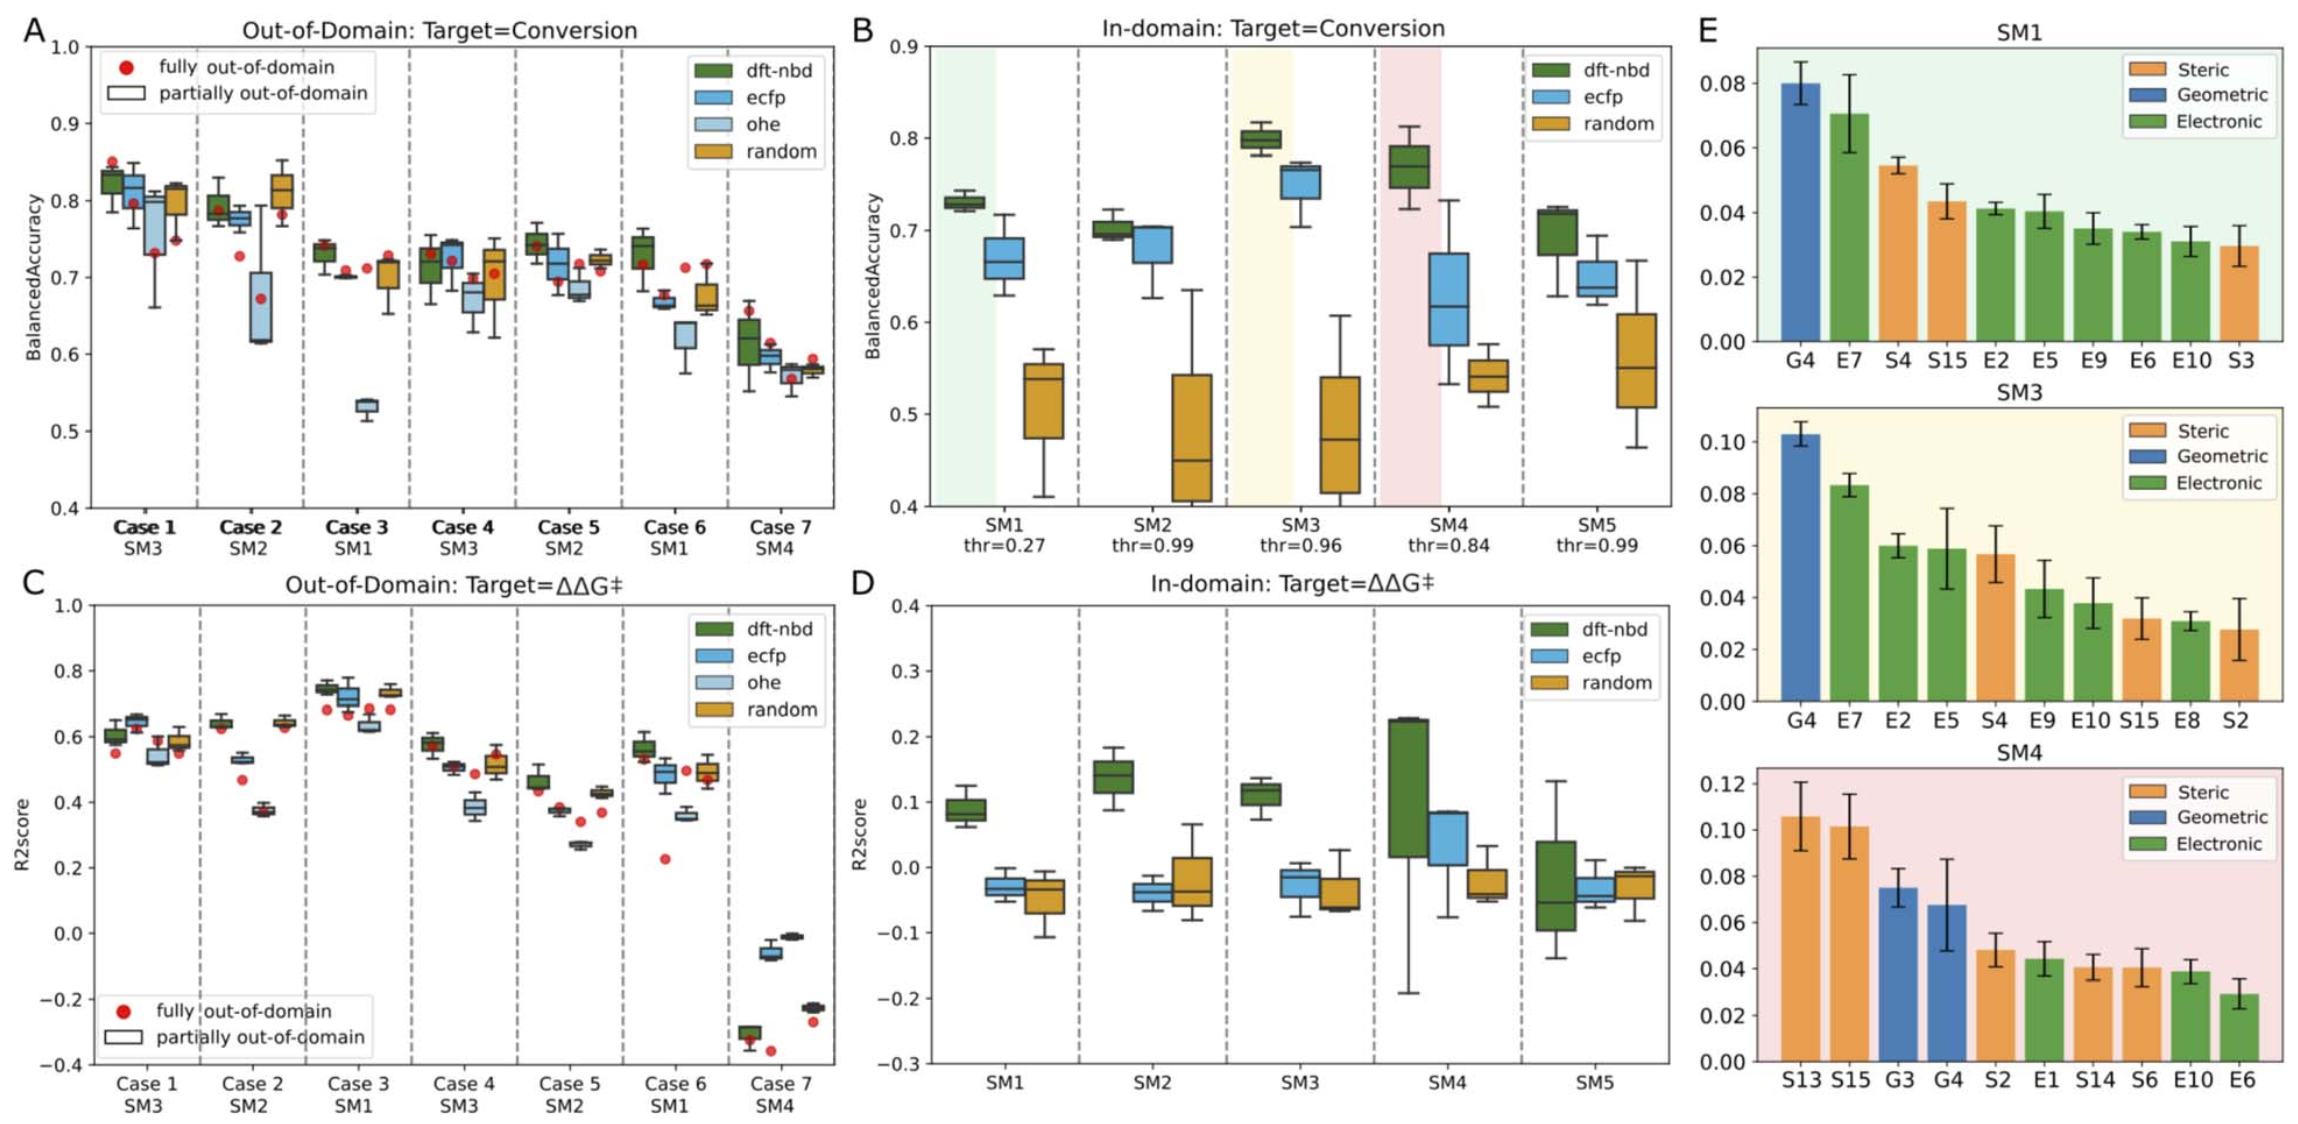
\includegraphics[width=\textwidth]{figures/CH5-pidko3.png}

  \caption{Performance metrics for asymmetric hydrogenation modelling. The coloured panels show feature importance for the in-domain classifiers trained on DFT descriptors.}
  \label{fig5:pidko3}
\end{figure}

\begin{figure}[htbp]
  \centering
  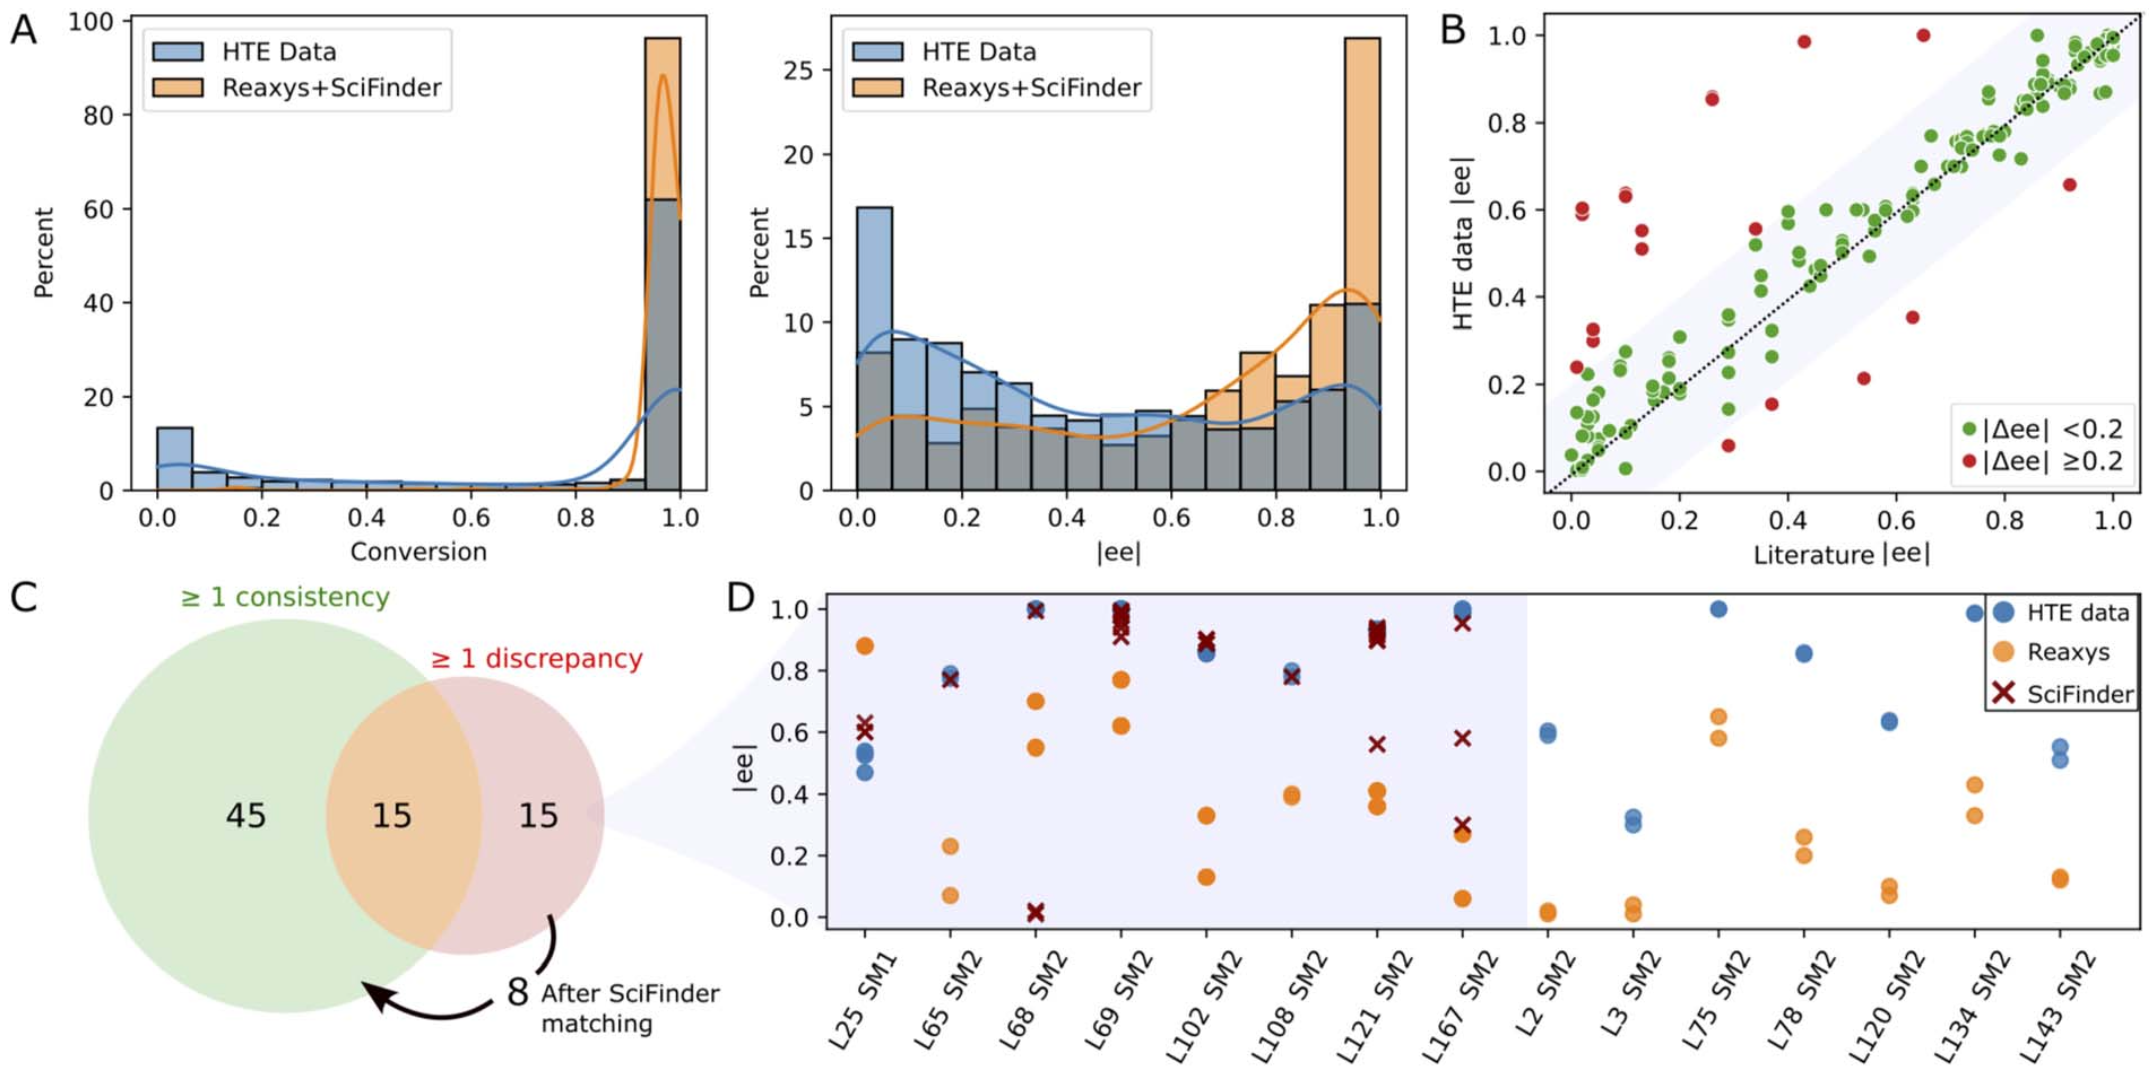
\includegraphics[width=\textwidth]{figures/CH5-pidko-data.png}
  \caption{Comparison of the high-throughput experimental data with the literature.}
  \label{fig5:pidko-data}
\end{figure}

The dataset contained many more negative or poor outcomes than the corresponding literature record (Fig.~\ref{fig5:pidko-data}), demonstrating again how publication and selection practices alter the response distribution seen by a model.
In the next chapter, we will discuss approaches for robust and high-throughput data collection.

\section{When should a prediction be trusted?}

\solution{5cm}{%
\begin{itemize}
  \item Define an applicability domain in chemical languate.
  \item Interpolation, response/representation extrapolation.
  \item Random reaction split can place nearly identical chemistry in training and test sets.
  \item Component-held-out or scaffold-held-out tests.
  \item Reaction in same mechanistic regime as data? 
  \vspace{1em}

  \keypoint{An unseen experiment is not necessarily unseen chemistry},
\end{itemize}
}

Predictive success shows that a relationship is useful for estimating a response over a tested domain.
Mechanistic explanation requires evidence that the proposed variables and causal story survive intervention and independent measurement.
A descriptor may be important because it correlates with the true controlling variable, because it identifies a family of molecules, or because it leaks information about the response.

\solution{6cm}{
\begin{itemize}
  \item \keypoint{Prediction is not mechanistic interpretation!}
 \vspace{2em}
  \item Correlated descriptors can exchange apparent importance without changing model performance.
  \item Orthogonal measurement before mechanistic claims.
  \item Chemistry determines if we can trust the model.
\end{itemize}
}

The most productive modelling studies use prediction and chemical interpretation together.
They report the domain, validation design, residuals, and failures, and they use surprising predictions to motivate new experiments.